%-----------------------------------------------------------------------------%
\chapter{\babEmpat} \label{chap:analisis}
%-----------------------------------------------------------------------------%%-----------------------------------------------------------------------------%
\section{Pendahuluan}
%-----------------------------------------------------------------------------%
Pada bab ini, analisis korpus data jurnalistik Bahasa Indonesia termutakhir ragam tulis dan lisan dijabarkan melalui beberapa tahap. Kedua korpus dianalisis secara terpisah agar temuan analisis dapat disandingkan untuk melihat perbedaan karakter serta signifikansi perbedaan tersebut antara data ragam tulis dan ragam lisan. Tahap pertama merupakan proses penguraian kalimat dengan metode komputasional berdasarkan dependensinya. Merujuk pada penjelasan dalam \autoref{chap:metode_penelitian}, penguraian kalimat ini dilakukan dengan bantuan sebuah kerangka kerja yang dapat dilatih ulang untuk pengkategorian token, penguraian lemma, dan penguraian kalimat bernama UDPipe (Straka & Strakov�, 2017). Tahap kedua adalah percobaan acak dengan metode Free Word Order Baseline (Futrell dkk, 2015) terhadap tabel yang dihasilkan oleh tahap pertama. Kemudian, pada tahap ketiga dilakukan proses penghitungan untuk mendapatkan nilai-nilai Panjang Dependensi atau Dependency Length  (DL) dan Rata-rata Jarak Dependensi atau Mean Dependency Distance (MDD) yang melibatkan proses agregasi atau pengelompokan data dan penerapan logika perhitungan untuk mendapatkan nilai DL yang diadopsi dari penelitian Futrell dkk (2015) dan MDD yang diadopsi dari penelitian Liu dkk (2017). Tahap keempat atau terakhir melibatkan analisis secara kualitatif terhadap kalimat-kalimat di dalam kedua korpus yang mewakili aspek-aspek temuan penelitian.

Pada tahap pertama, kedua korpus data jurnalistik dipersiapkan untuk dapat diolah dengn metode komputasional. Dalam data ragam lisan ditemukan beberapa ujaran yang bersifat tidak selesai. Ujaran seperti ini dihilangkan terlebih dahulu agar tidak mempengaruhi hasil penghitungan ujaran lainnya. Hasil dari tahap penguraian kalimat ini berupa tabel yang berisi anotasi konstituen-konstituen ujaran seperti contoh pada Tabel 1. Berdasarkan penguraian kalimat ini, kedua korpus memiliki total 19.530 kalimat atau 270.409 konstituen dengan data ragam tulis berjumlah 9311 kalimat atau 162.201 konstituen dan data ragam lisan berjumlah 10.219 kalimat atau 108.208 konstituen. Untuk memastikan kualitas penguraian kalimat dan anotasi yang sesuai, dilakukan tahap tambahan yaitu pemeriksaan secara manual. Berdasarkan pemeriksaan ini, kualitas penguraian kalimat untuk data ragam tulis terbilang sudah bagus, namun pada ragam lisan masih diperlukan pengembangan terutama untuk kata-kata informal atau sehari-hari. Contoh hasil penguraian pada \tab~\ref{tab:penggalan_kalimat} memperlihatkan ujaran "Mengingat fungsi dari telepon seluler tersebut sebagai sarana komunikasi yang berdampak pada peningkatan ekonomi" yang telah diekstraksi menjadi kata-kata yang memiliki anotasi untuk kelas kata serta hubungan antarkonstituennya. 

\begin{center}
\begin{table} \caption{Penggalan penguraian kalimat diambil dari korpus yang dianalisis}\label{tab:penggalan_kalimat}
\begin{tiny}
  \begin{tabulary}{1\textwidth}{| L | L | L | L | L | L | L |}
  \hline
    type & sentence & token & upos & relation & token id & head token id \\ \hline
tulis & Mengingat fungsi dari telepon seluler tersebut sebagai sarana komunikasi yang berdampak pada peningkatan perekonomian & Mengingat & VERB & root & 1 & 0 \\ \hline
tulis & Mengingat fungsi dari telepon seluler tersebut sebagai sarana komunikasi yang berdampak pada peningkatan perekonomian & fungsi & NOUN & obj & 2 & 1 \\ \hline
tulis & Mengingat fungsi dari telepon seluler tersebut sebagai sarana komunikasi yang berdampak pada peningkatan perekonomian & dari & ADP & case & 3 & 4 \\ \hline
tulis & Mengingat fungsi dari telepon seluler tersebut sebagai sarana komunikasi yang berdampak pada peningkatan perekonomian & telepon & NOUN & adl & 4 & 2 \\ \hline
tulis & Mengingat fungsi dari telepon seluler tersebut sebagai sarana komunikasi yang berdampak pada peningkatan perekonomian & seluler & NOUN & compound & 5 & 4 \\ \hline
tulis & Mengingat fungsi dari telepon seluler tersebut sebagai sarana komunikasi yang berdampak pada peningkatan perekonomian & tersebut & DET & det & 6 & 4 \\ \hline
tulis & Mengingat fungsi dari telepon seluler tersebut sebagai sarana komunikasi yang berdampak pada peningkatan perekonomian & sebagai & ADP & case & 7 & 8 \\ \hline
tulis & Mengingat fungsi dari telepon seluler tersebut sebagai sarana komunikasi yang berdampak pada peningkatan perekonomian & sarana & NOUN & adl & 8 & 2 \\ \hline
tulis & Mengingat fungsi dari telepon seluler tersebut sebagai sarana komunikasi yang berdampak pada peningkatan perekonomian & komunikasi & NOUN & compound & 9 & 8 \\ \hline
tulis & Mengingat fungsi dari telepon seluler tersebut sebagai sarana komunikasi yang berdampak pada peningkatan perekonomian & yang & PRON & nsubj & 10 & 11 \\ \hline
tulis & Mengingat fungsi dari telepon seluler tersebut sebagai sarana komunikasi yang berdampak pada peningkatan perekonomian & berdampak & VERB & acl:relcl & 11 & 8 \\ \hline
tulis & Mengingat fungsi dari telepon seluler tersebut sebagai sarana komunikasi yang berdampak pada peningkatan perekonomian & pada & ADP & case & 12 & 13 \\ \hline
tulis & Mengingat fungsi dari telepon seluler tersebut sebagai sarana komunikasi yang berdampak pada peningkatan perekonomian & peningkatan & NOUN & obl & 13 & 11 \\ \hline
tulis & Mengingat fungsi dari telepon seluler tersebut sebagai sarana komunikasi yang berdampak pada peningkatan perekonomian & perekonomian & NOUN & compound & 14 & 13 \\ 
\hline
  \end{tabulary}  
\end{tiny}
\end{table}
\end{center}

Untuk memudahkan dalam analisis kualitatif dan melihat secara dekat tautan-tautan dependensi yang terbentuk pada sebuah ujaran, visualisasi seperti pada \pic~\ref{fig:visualisasi_penguraian} dilakukan secara terpisah. Proses visualisasi ini hanya dilakukan pada ujaran-ujaran yang akan dilihat lebih rinci sebagai contoh yang mewakili hasil temuan. Pada kalimat contoh ini, terlihat bahwa ujaran memiliki root verbal "Mengingat" yang simpai sentralnya hanya terdiri dari satu tautan, yaitu "Mengingat fungsi" dengan hubungan tautan obj atau obyek. Penelitian ini merupakan penelitian terhadap penggunaan bahasa secara nyata (real utterance). Sehingga,  meskipun beberapa ujaran yang ditemukan terlihat seperti klausa terikat saja, atau tampak seperti ujaran yang tidak lengkap, semua ujaran tetap dianalisis tanpa dimanipulasi.

\begin{figure}
	\centering 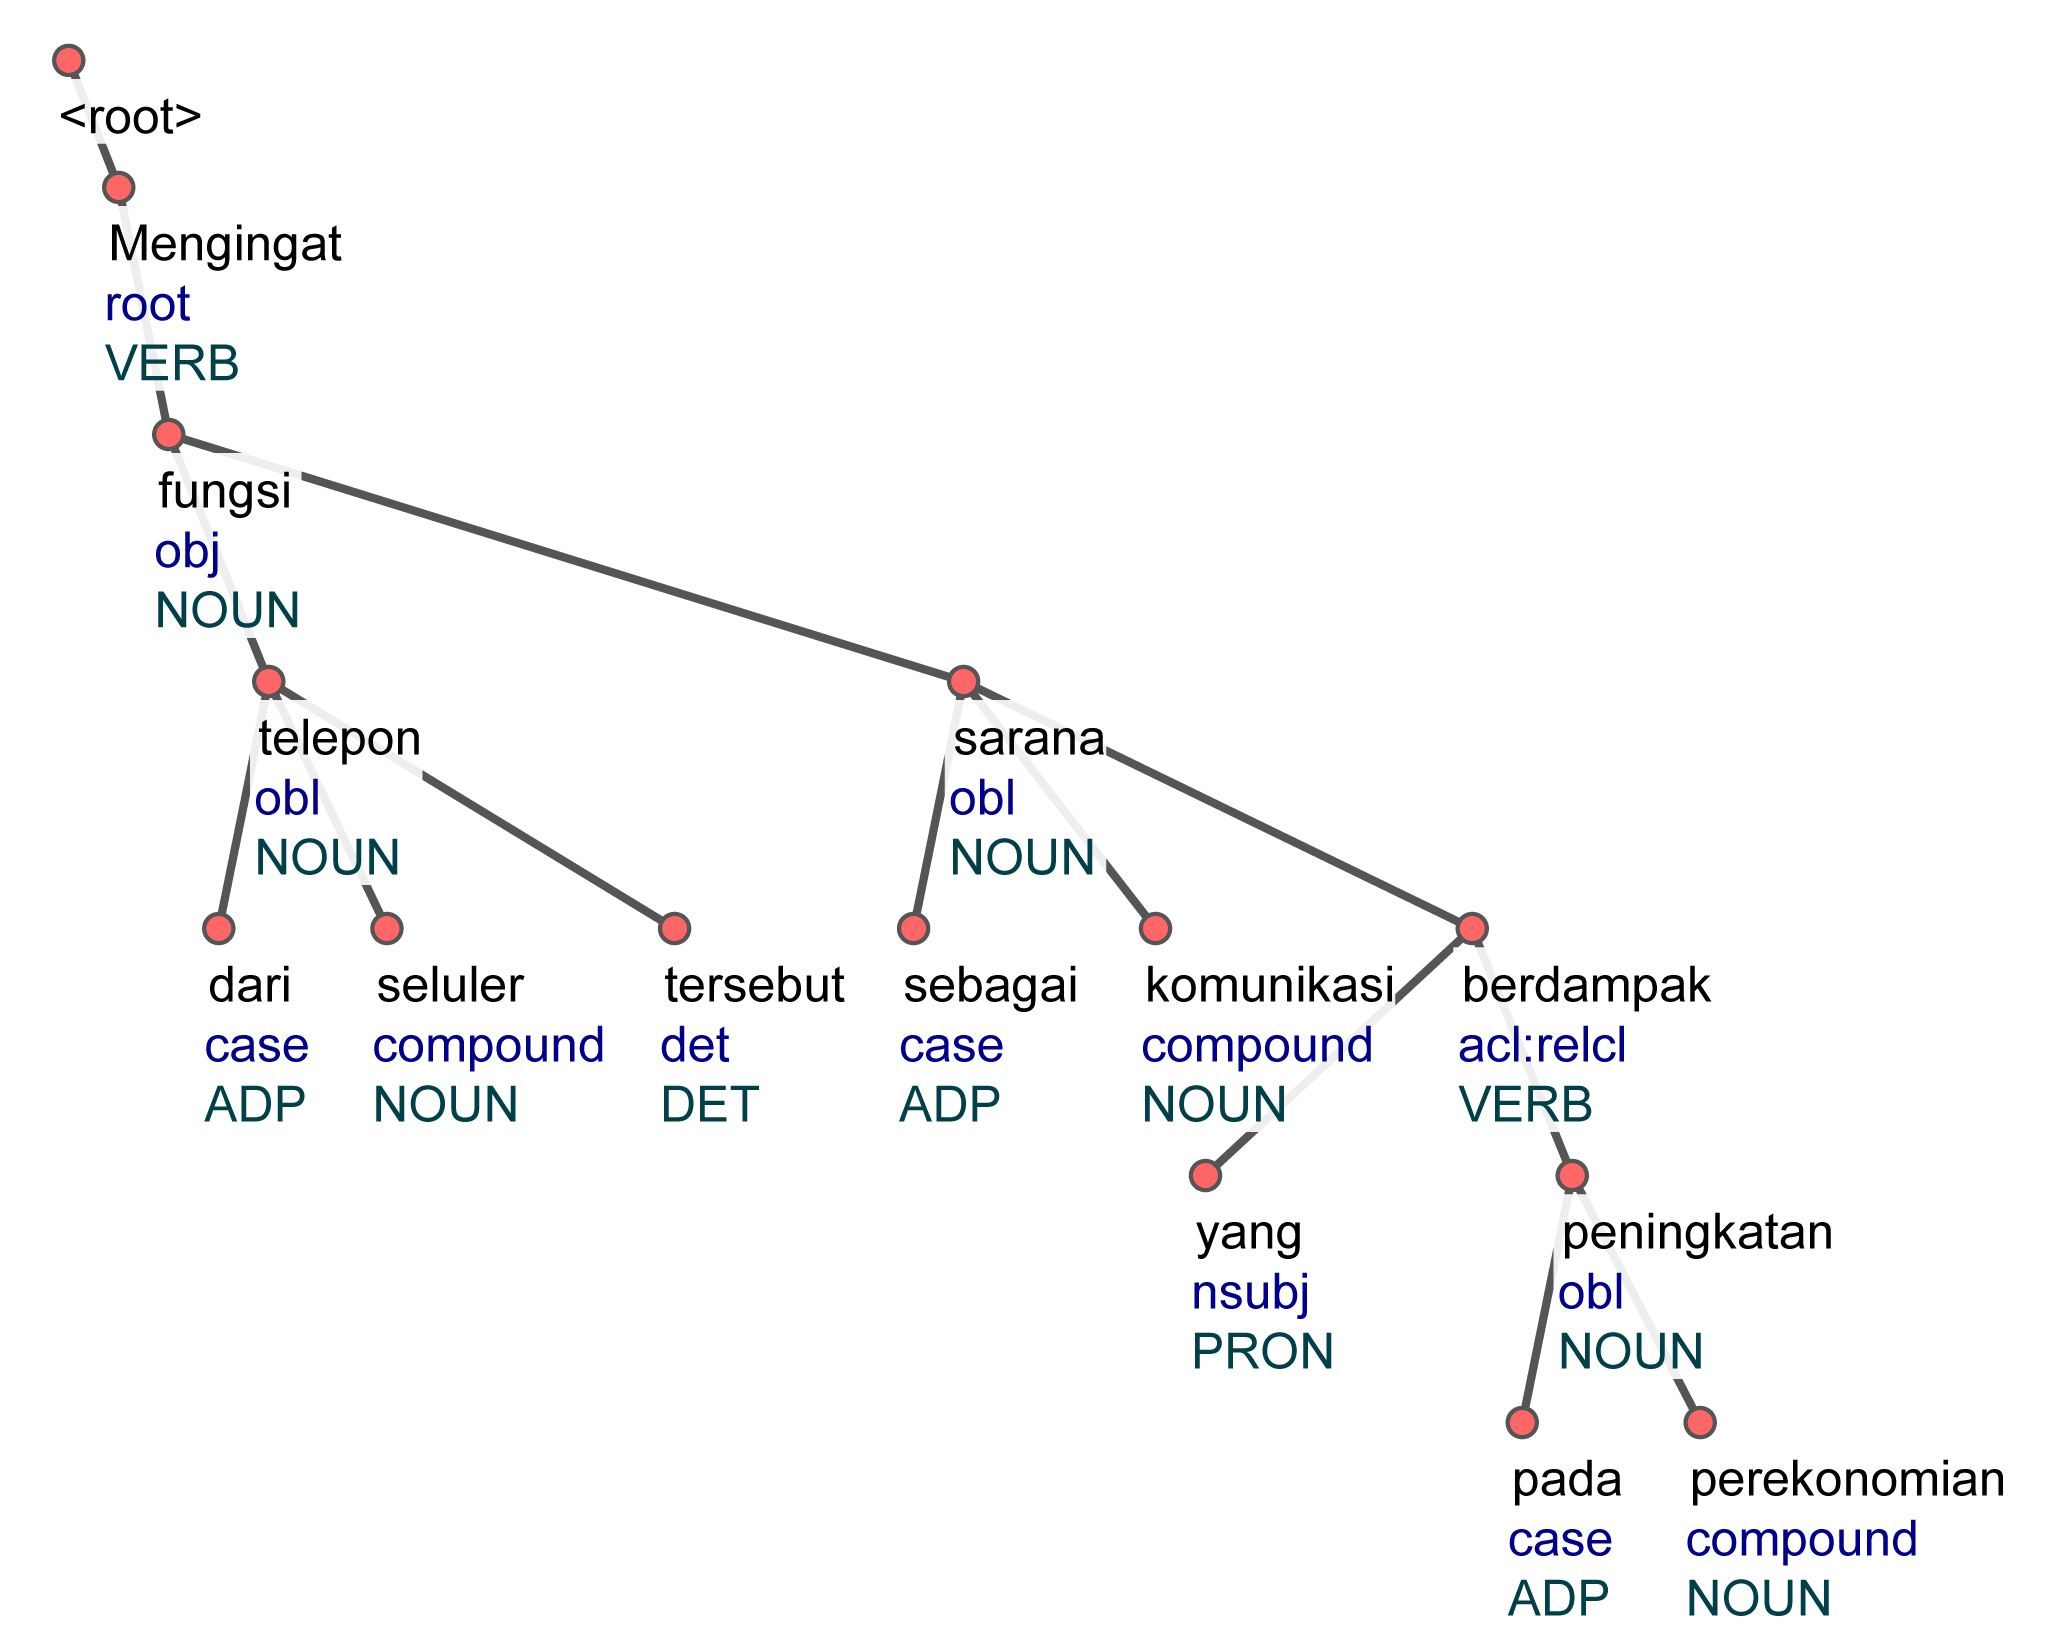
\includegraphics[width=1
	\textwidth] {pics/visualisasi_penguraian.jpg} 
	\caption{Contoh visualisasi penguraian kalimat berdasarkan dependensi} 
\label{fig:visualisasi_penguraian} \end{figure}

Tahap kedua yang dilakukan setelah mendapatkan tabel hasil penguraian ini adalah percobaan acak dengan acuan Free Word Order Baseline. Free Word Order Baseline merupakan pendekatan yang dilakukan untuk Futrell dkk (2015) dalam menguji hipotesis adanya Pengurangan Panjang Dependensi atau Dependency Length Minimization (DLM) yang juga berkaitan dengan Pengurangan Jarak Dependensi atau Dependency Distance Minimization (DDM). Dari ujaran-ujaran yang telah diurai, percobaan ini menghasilkan 100 kombinasi struktur ujaran dengan mempertahankan tautan dependensi sesuai hasil observasi. \pic~\ref{fig:percobaan_acak} memperlihatkan 3 contoh hasil percobaan acak terhadap kalimat "Sama, nanti pecahannya kita lihat" dan perbedaan nilai DL yang didapatkan 3 kombinasi struktur lainnya. Percobaan acak ini dilakukan terhadap semua ujaran yang berada pada kategori jumlah konstituen dengan frekuensi terbanyak. Berdasarkan klasifikasi kalimat terhadap kedua korpus data dan tahap pertama analisis, frekuensi jumlah konstituen terbanyak pada setiap klasifikasi kalimat adalah 10 konstituen (tulis) dan 5 konstituen (lisan) untuk klasifikasi kalimat pendek (\textless= 10 konstituen), 14 konstituen (tulis) dan 12 konstituen (lisan) untuk klasifikasi kalimat menengah (11-20 konstituen), serta 21 konstituen (tulis) dan 22 konstituen (lisan) untuk klasifikasi kalimat panjang. 

\begin{figure}
	\centering 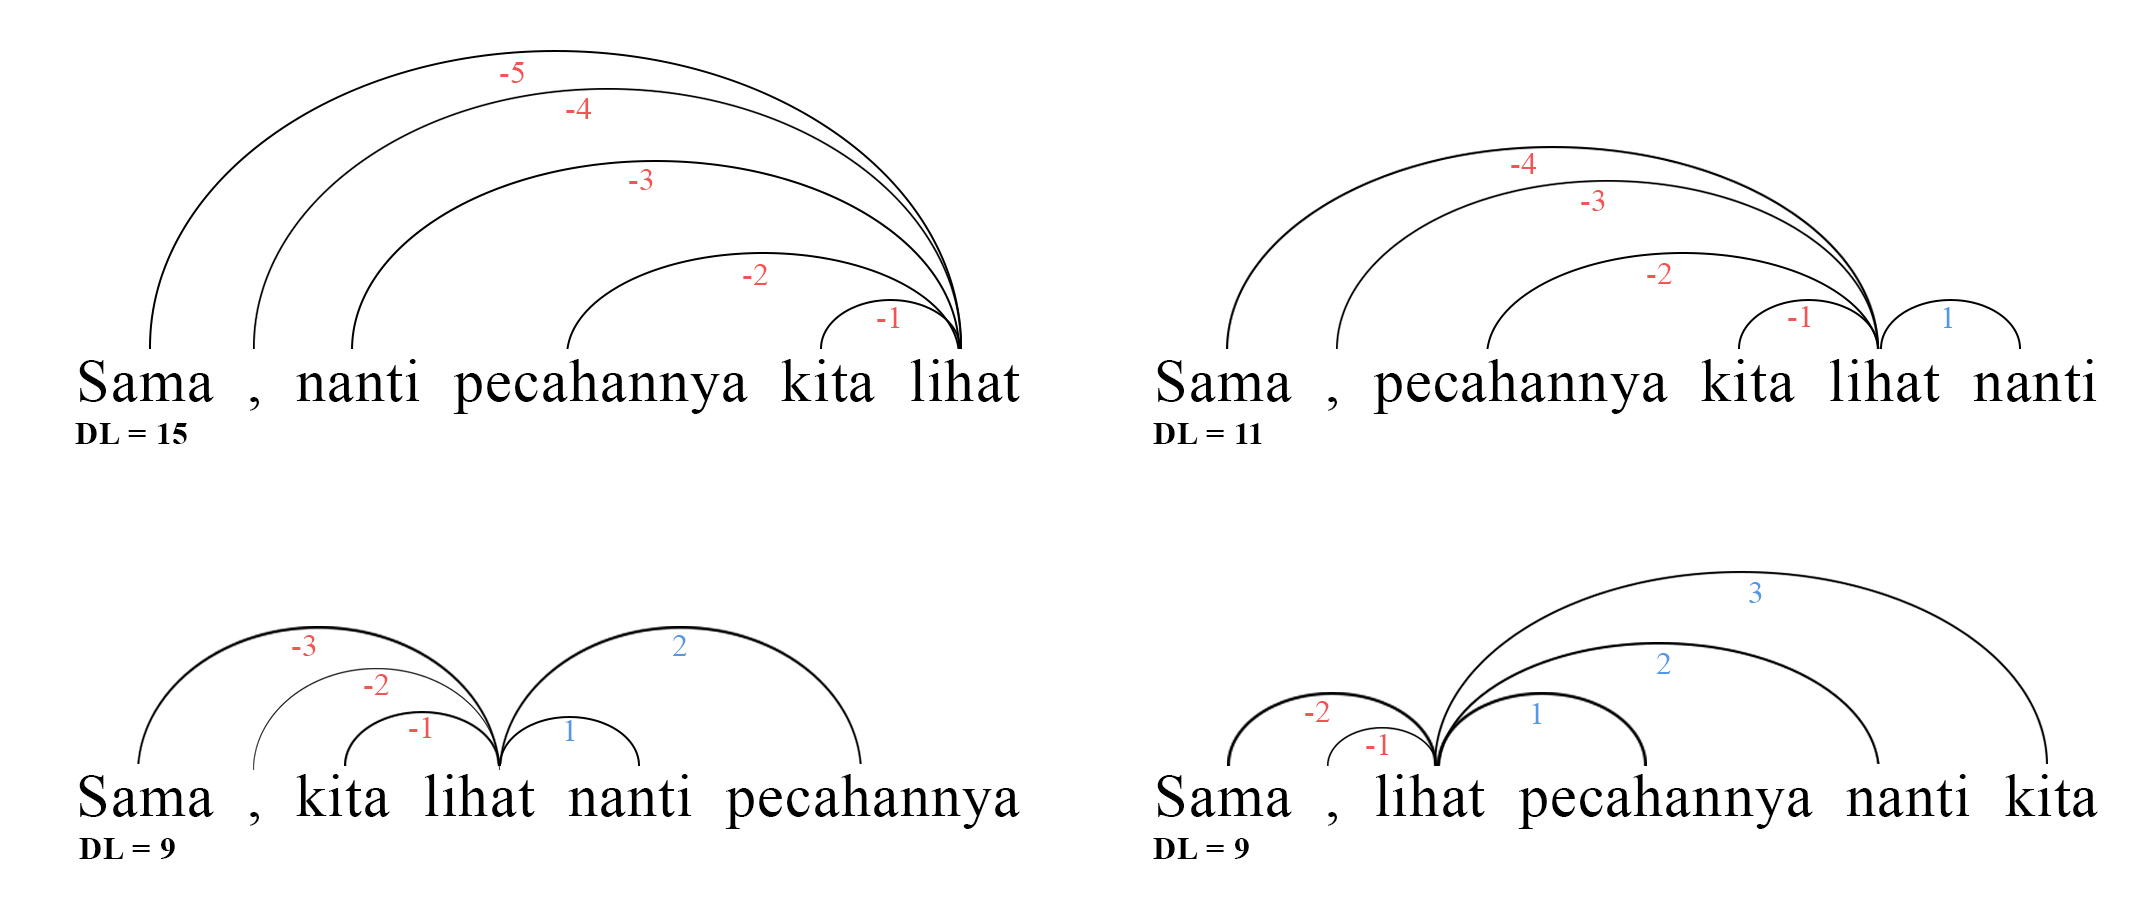
\includegraphics[width=1
	\textwidth] {pics/percobaan_acak.jpg} 
	\caption{Contoh hasil percobaan acak} 
\label{fig:percobaan_acak} 
\end{figure}

Merujuk pada penjelasan dalam tinjauan pustaka (Bab 2), Bahasa Indonesia memiliki urutan kata yang cenderung bebas, dan beberapa kasus menunjukkan pertukaran kata maupun klausa tidak mengubah makna ujaran (Sneddon, 2010). Dalam penelitiannya, Futrell dkk (2015) menunjukkan kedekatan hasil data observasi Bahasa Indonesia dengan nilai minimum menggunakan pendekatan ini untuk korpus data yang berisi tulisan penelitian. Temuan ini memberikan indikasi bahwa penerapan kebebasan urutan kata tidak hanya terjadi pada ujaran yang dianggap gramatikal, tetapi terutama pada penggunaan bahasa secara nyata dalam kehidupan sehari-hari (performance). Kebebasan terhadap aturan ini dan asumsi bahwa penutur Bahasa Indonesia memanfaatkan kebebasan ini merupakan dasar utama pemilihan pendekatan Free Word Order Baseline. Hal ini dikarenakan pendekatan tersebut menghasilkan hasil kombinasi struktur ujaran yang paling minimum dan maksimum sehingga sangat menarik untuk melihat posisi real utterance yang didapat melalui observasi terhadap kemungkinan kombinasi struktur yang ada. 

Tahap ketiga melibatkan proses anotasi untuk nilai-nilai yang berkaitan dengan tautan dependensi sebuah ujaran. Anotasi ini dihasilkan melalui penghitungan nilai DL dan penghitungan nilai MDD seperti yang dijabarkan pada Bab 2 dan 3. DL menekankan pada total jumlah dependensi yang didapatkan dari semua tautan dependensi dalam sebuah ujaran, sedangkan MDD menekankan pada rata-rata jarak dependensi antara dua konstituen dalam sebuah ujaran. Meskipun memiliki prinsip mendasar yang serupa, saya berasumsi ada perbedaan informasi yang berarti antara kedua pendekatan ini sehingga keduanya digunakan dalam penelitian ini. Eksplorasi perbedaan pendekatan DL dan MDD serta penentuan pendekatan mana yang lebih optimal dalam mengilustrasikan efisiensi memori kerja melalui struktur sintaksis ujaran bukan merupakan fokus penelitian ini, namun hasil penerapan kedua pendekatan dalam penelitian ini dapat berkontribusi dalam menunjukkan pada kondisi mana kedua pendekatan tersebut berbeda.

\begin{center}
\begin{table} \caption{Penggalan penguraian kalimat diambil dari korpus yang dianalisis}\label{tab:dl_mdd}
\begin{tiny}
  \begin{tabulary}{1\textwidth}{| L | L | L | L | L | L | L | L |}
  \hline
type & sentence & dl & sum\textunderscore dl & dl\textunderscore positive & dl\textunderscore negative & mdd \\ \hline
tulis & Mengingat fungsi dari telepon seluler tersebut sebagai sarana komunikasi yang berdampak pada peningkatan perekonomian & 0 & 0 & 0 & 0 & 0.00 \\ \hline
tulis & Mengingat fungsi dari telepon seluler tersebut sebagai sarana komunikasi yang berdampak pada peningkatan perekonomian & 1 & 1 & 1 & 0 & 0.08 \\ \hline
tulis & Mengingat fungsi dari telepon seluler tersebut sebagai sarana komunikasi yang berdampak pada peningkatan perekonomian & -1 & 2 & 1 & -1 & 0.15 \\ \hline
tulis & Mengingat fungsi dari telepon seluler tersebut sebagai sarana komunikasi yang berdampak pada peningkatan perekonomian & 2 & 4 & 3 & -1 & 0.31 \\ \hline
tulis & Mengingat fungsi dari telepon seluler tersebut sebagai sarana komunikasi yang berdampak pada peningkatan perekonomian & 1 & 5 & 4 & -1 & 0.38 \\ \hline
tulis & Mengingat fungsi dari telepon seluler tersebut sebagai sarana komunikasi yang berdampak pada peningkatan perekonomian & 2 & 7 & 6 & -1 & 0.54 \\ \hline
tulis & Mengingat fungsi dari telepon seluler tersebut sebagai sarana komunikasi yang berdampak pada peningkatan perekonomian & -1 & 8 & 6 & -2 & 0.62 \\ \hline
tulis & Mengingat fungsi dari telepon seluler tersebut sebagai sarana komunikasi yang berdampak pada peningkatan perekonomian & 6 & 14 & 12 & -2 & 1.08 \\ \hline
tulis & Mengingat fungsi dari telepon seluler tersebut sebagai sarana komunikasi yang berdampak pada peningkatan perekonomian & 1 & 15 & 13 & -2 & 1.15 \\ \hline
tulis & Mengingat fungsi dari telepon seluler tersebut sebagai sarana komunikasi yang berdampak pada peningkatan perekonomian & -1 & 16 & 13 & -3 & 1.23 \\ \hline
tulis & Mengingat fungsi dari telepon seluler tersebut sebagai sarana komunikasi yang berdampak pada peningkatan perekonomian & 3 & 19 & 16 & -3 & 1.46 \\ \hline
tulis & Mengingat fungsi dari telepon seluler tersebut sebagai sarana komunikasi yang berdampak pada peningkatan perekonomian & -1 & 20 & 16 & -4 & 1.54 \\ \hline
tulis & Mengingat fungsi dari telepon seluler tersebut sebagai sarana komunikasi yang berdampak pada peningkatan perekonomian & 2 & 22 & 18 & -4 & 1.69 \\ \hline
tulis & Mengingat fungsi dari telepon seluler tersebut sebagai sarana komunikasi yang berdampak pada peningkatan perekonomian & 1 & 23 & 18 & -5 & 1.77 \\ \hline
  \end{tabulary}  
\end{tiny}
\end{table}
\end{center}

\tab~\ref{tab:dl_mdd} memperlihatkan penghitungan nilai DL dan MDD untuk kalimat "Mengingat fungsi dari telepon seluler tersebut sebagai sarana komunikasi yang berdampak pada peningkatan perekonomian". Dengan jumlah konstituen 14, kalimat ini memiliki nilai DL 23 dan MDD 1,77. Hasil ini menunjukkan semua nilai tautan dependensi dalam ujaran tersebut berjumlah 23 dengan rata-rata jarak dependensi antarkonstituen yang memiliki tautan langsung sejauh 1,77 konstituen. Pada tabel tersebut terlihat bahwa nilai DL juga dipisahkan menjadi dua berdasarkan arahnya. Nilai DL positif menggambarkan kondisi head-initial yang berarti konstituen terikat (dependant) direalisasikan setelah konstituen induk (root/head). Sebaliknya, nilai DL negatif menggambarkan kondisi head-final yang berarti dependant direalisasikan sebelum root. Analisis hubungan nilai DL positif dan negatif ini memiliki dua bagian. Bagian pertama melihat tautan antara 2 konstituen yang memiliki tautan langsung tanpa memperhitungkan posisi frasa atau klausa kedua konstituen tesebut. Analisis bagian kedua melihat tautan antara 2 konstituen di mana salah satu konstituen tersebut adalah root verbal (simpai sentral) dan menganggap semua simpai cabang konstituen tersebut mengikuti nilainya. Pada kalimat kompleks yang memiliki lebih dari 1 klausa, tautan dependensi utama ini dapat membawa 1 klausa atau lebih di dalamnya. Sebagai contoh, jika terdapat 1 tautan dependensi utama yang negatif, dan dalam simpai cabang tersebut terdapat 2 klausa, maka kedua klausa tersebut harus disimpan di dalam memori kerja terlebih dahulu hingga root direalisasikan dan hal ini memberatkan memori kerja sehingga menjadikan komunikasi lebih sulit. Analisis ini berangkat dari asumsi bahwa Bahasa Indonesia cenderung memilih bentuk tautan head-initial yang diambil dari indikasi dari teori setruktur frasa yang mengungkapkan banyaknya kondisi di mana head akan mendahului konstituen terikatnya (Kridalaksana, 2002; Sneddon, 2010).

Tahap keempat atau terakhir merupakan analisis kualitatif untuk melihat perubahan valensi kata difokuskan pada valensi verbal pada simpai sentral ujaran. Verba sebagai root ujaran ditemukan sebanyak 84,67\% atau sebanyak 7884 ujaran pada data ragam tulis dan 69,26\% atau sebanyak 7078 ujaran pada data ragam lisan. Analisis ini dilakukan untuk melihat adanya strategi yang menyebabkan terjadinya DLM dan DDM pada level paling utama (simpai sentral) serta perbedaan karakter yang mungkin muncul antara kedua jenis ragam bahasa.

%-----------------------------------------------------------------------------%
\section{Panjang Dependensi atau Dependency Length (DL) dan Rata-rata Jarak Dependensi atau Mean Dependency Distance (MDD) pada Data Jurnalistik Ragam Lisan dan Tulis}
%-----------------------------------------------------------------------------%
Pada analisis penelitian ini, kedua pendekatan untuk menghitung nilai DL dan nilai MDD digunakan karena diduga masing-masing memberikan informasi yang berbeda atau menunjukkan perbedaan nilai pada kondisi tertentu. Kedua penghitungan ini dilakukan terhadap setiap ujaran dalam korpus data jurnalistik ragam lisan dan tulis. Secara garis besar, ada perbedaan yang cukup terlihat dalam kedua paparan grafik nilai DL dan nilai MDD antara korpus data ragam tulis dan data ragam lisan.

%-----------------------------------------------------------------------------%
\subsection{Perbandingan nilai Panjang Dependensi atau Dependency Length (DL) antara data ragam tulis dan data ragam lisan}
%-----------------------------------------------------------------------------%
Pada pendekatan penghitungan Panjang Dependensi atau Dependency Length (DL) yang diadopsi dari penelitian Futrell dkk (2015), seluruh nilai tautan dependensi dalam sebuah ujaran dijumlahkan sehingga nilai DL yang dihasilkan cukup sensitif dan berbanding linear dengan jumlah konstituen dalam ujaran. Pada \pic~\ref{fig:lisantulis_DL} dapat dicermati bahwa terjadi perubahan pada kedua garis regresi. Perbandignan umum ini dilakukan tanpa melihat lebih dalam persebaran data terkait jumlah konstituen dalam ujaran atau tanpa memperhitungkan klasifikasi panjang kalimat. Berdasarkan grafik nilai DL ini, terlihat bahwa mayoritas jumlah konstituen dalam kalimat pada kedua korpus data berada di bawah 40 konstituen. Pada area di bawah 40 konstituen, garis regresi data ragam tulis berada di bawah garis regresi data ragam lisan. Namun, pada area di atas 40 konstituen, garis regresi menunjukkan perbandingan terbalik secara drastis. Secara umum, rata-rata nilai DL adalah 42,61 untuk data ragam tulis dan 24,36 untuk data ragam lisan. 

Secara kolektif tanpa memperhitungkan klasifikasi panjang kalimat, hasil tersebut menunjukkan adanya kecenderungan yang signifikan bahwa ragam lisan akan cenderung menghasilkan jumlah nilai tautan dependensi yang lebih kecil. Hal ini berarti ada indikasi bahwa data ragam lisan menunjukkan efisiensi yang lebih tinggi dibandingkan data ragam tulis dilihat dari segi total nilai dependensi dalam sebuah ujaran. Akan tetapi, seperti yang terlihat pada garis regresi yang terbentuk, hingga panjang kalimat 40 konstituen, garis regresi data ragam tulis terus berada di bawah garis regresi ragam lisan dan terjadi pemusatan data pada panjang kalimat yang mendekati minimum untuk data ragam lisan. Hal ini menunjukkan bahwa dugaan awal ini harus dicermati lebih dalam dengan melihat klasifikasi panjang kalimat yang mungkin akan memberikan informasi tambahan lain yang lebih menentukan keakuratan hasil uji hipotesis. 

\begin{figure}
	\centering 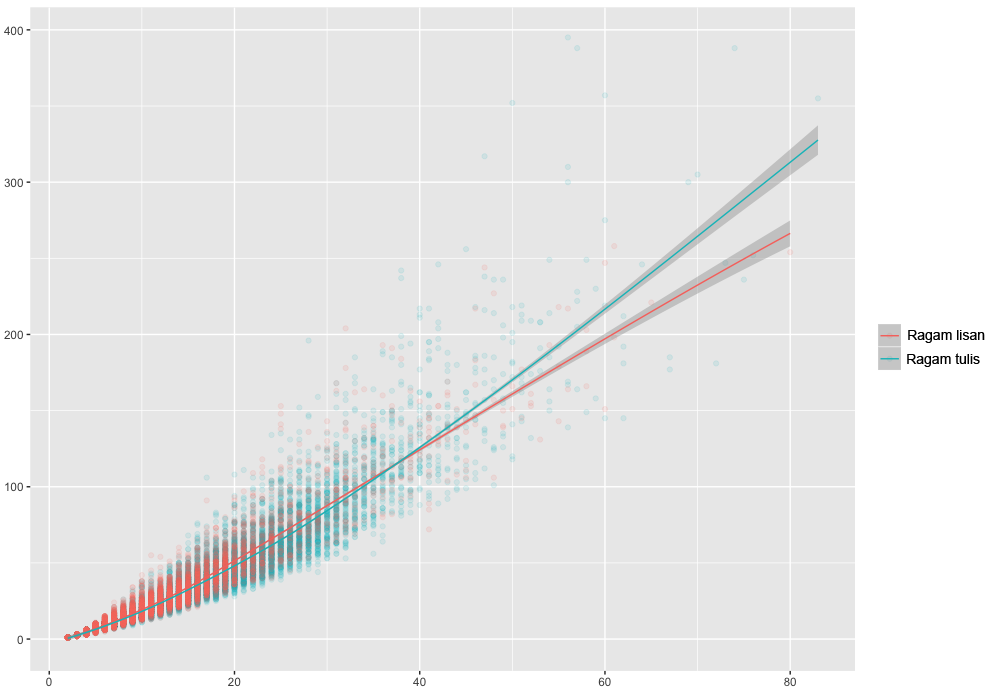
\includegraphics[width=1
	\textwidth] {pics/lisantulis_DL.png} 
	\caption{Grafik nilai DL data ragam tulis dan lisan} 
\label{fig:lisantulis_DL} 
\end{figure}

%-----------------------------------------------------------------------------%
\subsection{Perbandingan nilai Rata-rata Jarak Dependensi atau Mean Dependency Distance (MDD) antara data ragam tulis dan data ragam lisan}
%-----------------------------------------------------------------------------%
Berbeda dengan penghitungan nilai DL, Rata-rata Jarak Dependensi atau Mean Dependency Distance (MDD) didapatkan dengan membagi total nilai tautan dependensi dalam sebuah ujaran dengan jumlah tautan itu sendiri. Penghitungan ini menghasilkan perkiraan rata-rata jarak dependensi satu (1) tautan dalam sebuah ujaran sehingga menggambarkan pada umumnya sejauh apa jarak relasi semantik antar dua konstituen. Seperti \pic~\ref{fig:lisantulis_DL}, \pic~\ref{fig:lisantulis_MDD} merupakan paparan nilai MDD untuk semua kalimat pada kedua korpus data (ragam tulis dan lisan). Nilai MDD, seperti yang dikemukakan oleh Liu dkk (2017), tidak terlalu sensitif terhadap jumlah konstituen karena merupakan nilai rata-rata per tautan. Meskipun begitu, pada data dengan jumlah konstituen di bawah 10, nilai MDD masih menunjukkan hasil yang sangat linier terhadap jumlah konstituen. Apabila nilai DL memberikan gambaran umum mengenai kompleksitas sebuah ujaran karena hanya fokus terhadap total nilai, nilai MDD dapat lebih memberikan ilustrasi kerja kognisi yang tercermin pada relasi dua buah konstituen di mana untuk kedua konstituen dapat diproses, salah satu harus menunggu yang lain untuk direalisasikan. Pada Gambar 4, dapat disimpulkan bahwa garis regresi untuk korpus data ragam tulis juga berada di bawah garis regresi korpus data ragam lisan dengan panjang kalimat di bawah 40 konstituen namun berbanding terbalik setelah 40 konstituen. Temuan ini menunjukkan konsistensi antara nilai DL dan nilai MDD yang sama-sama menunjukkan bahwa hingga jumlah setidaknya 40 konstituen, kalimat-kalimat dalam data ragam tulis menunjukkan efisiensi yang lebih tinggi dari segi dependensi dibandingkan data ragam lisan. Namun, rata-rata nilai MDD yang didapat adalah 2,05 konstituen untuk data ragam lisan dan 2,35 konstituen untuk data ragam tulis. Seperti pada catatan grafik nilai DL sebelumnya, nilai ini tidak memperhitungkan klasifikasi panjang kalimat dan pemusatan data ragam tulis pada panjang kalimat yang mendekati minimum juga patut diperhitungkan.

\begin{figure}
	\centering 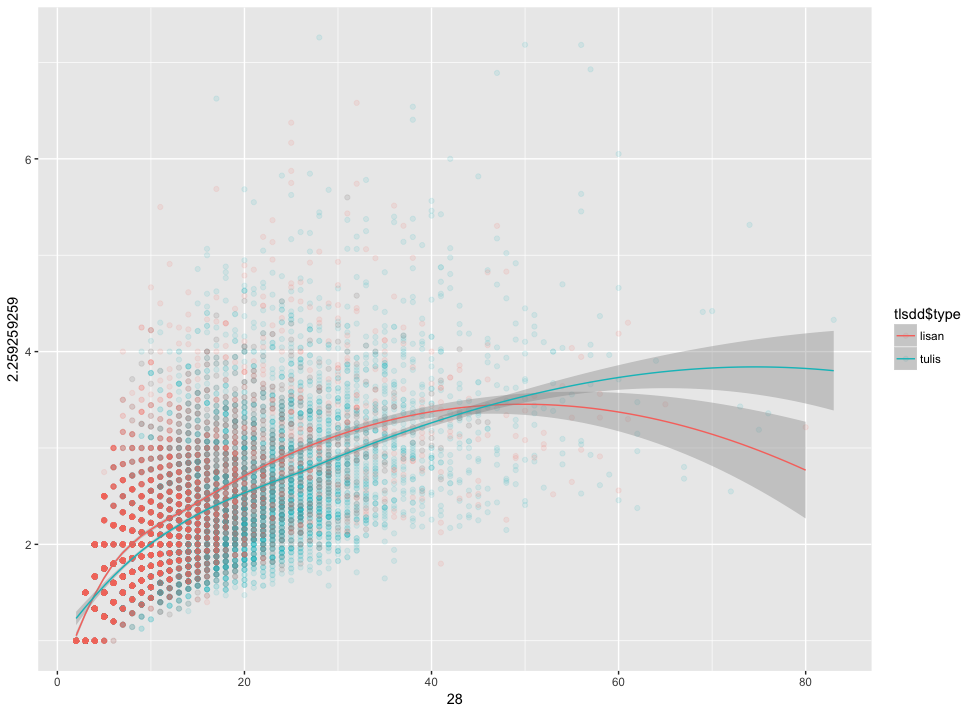
\includegraphics[width=1
	\textwidth] {pics/lisantulis_MDD.png} 
	\caption{Grafik nilai MDD data ragam tulis dan lisan} 
\label{fig:lisantulis_MDD} 
\end{figure}

%%-----------------------------------------------------------------------------%
\section{Perbandingan Nilai Data Hasil Observasi dengan Hasil Percobaan Acak}
%%-----------------------------------------------------------------------------%
Setelah mendapatkan gambaran umum mengenai nilai DL dan MDD untuk kedua korpus data, percobaan acak terhadap kedua korpus data dilakukan untuk melihat apakah ujaran-ujaran dalam data hasil observasi, baik ragam tulis maupun lisan, memiliki kecenderungan untuk menghindari nilai tautan dependensi yang lebih besar. Berdasarkan hipotesis DLM, Futrell dkk (2015) mengajukan bahwa jika bahasa berevolusi untuk mendukung komunikasi yang lebih mudah, maka seharusnya urutan kata yang dimanfaatkan penutur dalam penggunaan bahasa secara nyata sehingga tidak menghasilkan nilai panjang dependensi yang besar. Hal ini dikarenakan nilai panjang dependensi yang besar mencerminkan kompleksitas produksi ataupun pemahaman yang lebih tinggi. Percobaan acak dengan pendekatan Free Word Order Baseline menghasilkan 100 bentuk urutan kata acak dengan mempertahankan struktur tautan-tautan dependensi yang sama dengan ujaran dalam data observasi. Gambar 5 dan 6 menunjukkan grafik perbandingan antara nilai DL yang dihasilkan percobaan acak dan nilai DL dari semua ujaran dalam data observasi ragam tulis (\pic~\ref{fig:lisantulis_MDD}) serta ragam lisan (\pic~\ref{fig:lisantulis_MDD}). 

%%-----------------------------------------------------------------------------%
\subsection{Temuan 1: Pengurangan Panjang Dependensi atau Dependency Length Minimization (DLM) terjadi pada kedua korpus data}
%%-----------------------------------------------------------------------------%
\pic~\ref{fig:t10randomobs}, \pic~\ref{fig:t14randomobs},dan \pic~\ref{fig:t21randomobs} memperlihatkan histogram perbandingan nilai DL antara hasil percobaan acak dan data observasi untuk jumlah konstituen 10, 14, dan 21. Jumlah-jumlah konstituen ini memili frekuensi terbanyak mewakili setiap kelompok klasifikasi kalimat pada data ragam tulis.  Histogram hasil percobaan acak terlihat jelas membentuk kurva yang lebih rendah dibandingkan dengan kurva yang dibentuk oleh data observasi. Hal ini berarti a hasil percobaan acak memiliki distribusi nilai DL yang lebih besar dibandingkan dengan data observasi. Berdasarkan histogram ini, dapat dilihat juga bahwa pada jumlah konstituen yang semakin banyak, irisan antara kurva nilai DL data observasi dan hasil percobaan acak semakin sedikit.

\begin{figure}
	\centering 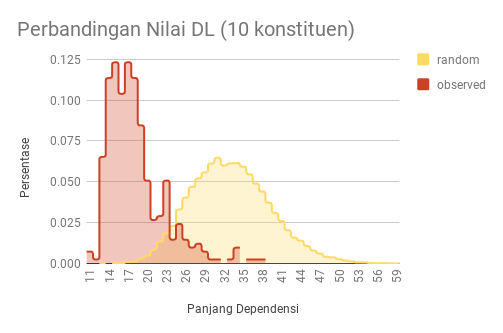
\includegraphics[width=1
	\textwidth] {pics/t10randomobs.png} 
	\caption{ nilai DL hasil percobaan acak dengan observasi untuk panjang kalimat 10 konstituen} 
\label{fig:t10randomobs} 
\end{figure}

\begin{figure}
	\centering 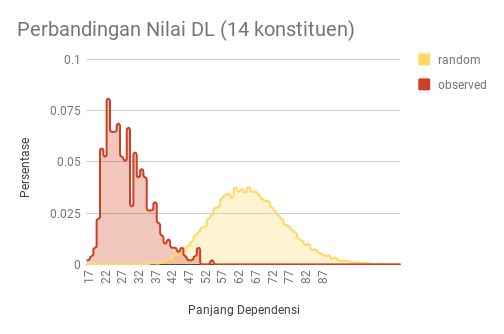
\includegraphics[width=1
	\textwidth] {pics/t14randomobs.png} 
	\caption{ nilai DL hasil percobaan acak dengan observasi untuk panjang kalimat 14 konstituen}\label{fig:t14randomobs} 
\end{figure}

\begin{figure}
	\centering 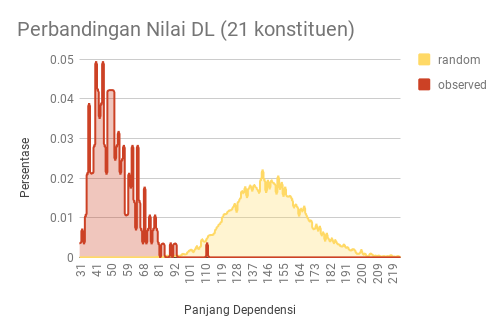
\includegraphics[width=1
	\textwidth] {pics/t21randomobs.png} 
	\caption{ nilai DL hasil percobaan acak dengan observasi untuk panjang kalimat 21 konstituen}\label{fig:t21randomobs} 
\end{figure}

\tab~\ref{tab:perbandingan_DL_tulis} menunjukkan perbedaan rata-rata nilai DL yang cukup jauh antara hasil percobaan acak dan data observasi untuk data ragam tulis dengan efek yang signifikan pada semua jumlah konstituen (P \textless 0,001). Tes signifikansi ini dilakukan dengan menerapkan pendekatan tes Stouffer.

\begin{center}
 \label{table:perbandingan_DL_tulis}
 \caption{Tabel perbandingan rata-rata nilai DL hasil percobaan acak dengan data observasi dan hasil tes signifikansi untuk data ragam tulis}
  \begin{tabular}{ | l | l |}
    \hline
    \hline
  \end{tabular}
\end{center}

Sesuai dengan ekspektasi, percobaan acak terhadap data ragam lisan menunjukkan hasil yang serupa dengan percobaan terhadap data ragam tulis. Gambar 6 merupakan histogram perbandingan nilai DL antara hasil percobaan acak dan data observasi untuk jumlah konstituen 5, 12, dan 22 yang mewakili setiap kelompok klasifikasi kalimat pada data ragam lisan. Histogram hasil percobaan acak untuk ragam lisan juga membentuk kurva yang secara jelas terlihat lebih rendah dan juga menandakan bahwa percobaan acak memiliki distribusi nilai DL yang lebih besar dibandingkan dengan data observasi. Bahkan untuk jumlah konstituen 5 yang tergolong kalimat sangat pendek, data observasi masih memperlihatkan adanya indikasi DLM secara signifikan dengan nilai P \textless 0,001. Berdasarkan histogram ini juga dapat disimpulkan bahwa pada jumlah konstituen yang semakin banyak, irisan antara nilai DL data observasi dan hasil percobaan acak semakin sedikit.

\begin{figure}
	\centering 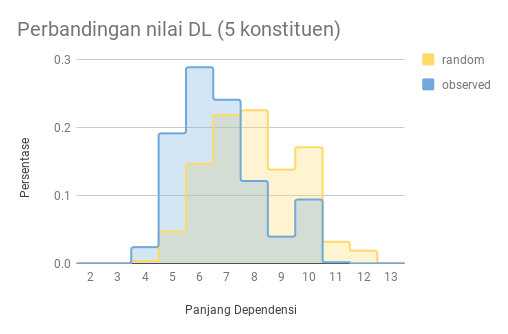
\includegraphics[width=1
	\textwidth] {pics/l5randomobs.png} 
	\caption{ Nilai DL hasil percobaan acak dengan hasil observasi untuk panjang kalimat 5 konstituen pada ragam lisan} 
	\label{fig:l5randomobs} 
\end{figure}

\begin{figure}
	\centering 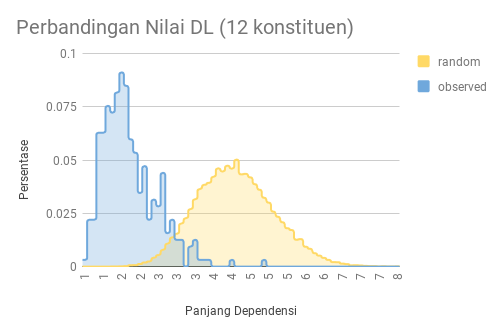
\includegraphics[width=1
	\textwidth] {pics/l12randomobs.png} 
	\caption{ Nilai DL hasil percobaan acak dengan hasil observasi untuk panjang kalimat 12 konstituen pada ragam lisan} 
	\label{fig:l12randomobs} 
\end{figure}

\begin{figure}
	\centering 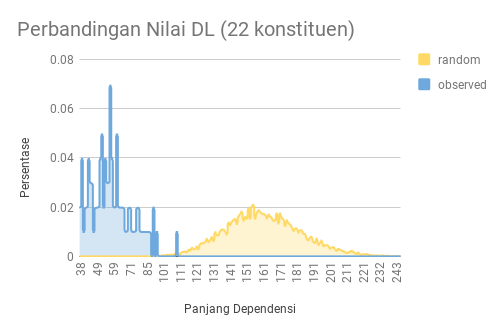
\includegraphics[width=1
	\textwidth] {pics/l22randomobs.png} 
	\caption{ Nilai DL hasil percobaan acak dengan hasil observasi untuk panjang kalimat 22 konstituen pada ragam lisan} 
	\label{fig:l22randomobs} 
\end{figure}

Serupa juga dengan percobaan terhadap data ragam tulis, \tab~\ref{tab:perbandingan_DL_lisan} menunjukkan perbedaan rata-rata nilai DL yang cukup jauh antara data observasi dan hasil percobaan acak untuk data ragam lisan dengan efek yang signifikan pada semua jumlah konstituen (P \textless 0,001).

\begin{center}
 \label{table:perbandingan_DL_lisan}
 \caption{Tabel perbandingan rata-rata nilai DL hasil percobaan acak dengan data observasi dan hasil tes signifikansi untuk data ragam lisan}
  \begin{tabular}{ | l | l |}
    \hline
    \hline
  \end{tabular}
\end{center}

Percobaan acak pada kedua korpus data dengan jumlah konstituen yang berbeda-beda menunjukkan adanya optimasi struktur ujaran pada data observasi sehingga terjadi pengurangan jarak dependensi (DLM) secara kolektif. Histogram hasil percobaan menunjukkan bahwa pada semua jumlah konstituen, distribusi nilai DL data observasi jauh lebih kecil mendekati jumlah minimum. Temuan ini sejalan dengan hipotesis penelitian Hawkins (2014) yang menyebutkan bahwa aturan urutan kata mendasar yang dalam pemahaman penutur akan menghasilkan konstruksi ujaran yang tautan dependensinya lebih pendek dibandingkan alternatif konstruksi yang mungkin ada.

%%-----------------------------------------------------------------------------%
\subsection{Diskusi Temuan I}
%%-----------------------------------------------------------------------------%
Hipotesis pengurangan panjang atau jarak dependensi (DLM atau DDM) berbicara tentang kecenderungan manusia untuk mendekatkan kata-kata yang memiliki relasi semantik. Pendekatan ini dapat dilakukan dengan menerapkan beberapa strategi seperti yang telah dibahas pada penelitian-penelitian terdahulu (Jaeger, 2006; Gildea & Temperley, 2015). Dalam ranah sintaksis, strategi pendekatan-kata-kata ini termasuk melalui penyusunan urutan kata dan pengurangan kata dalam kalimat (yang mungkin diakibatkan oleh pengurangan unsur yang repetitif ataupun hal yang lain). Berdasarkan tahap pertama analisis yaitu percobaan acak dengan menggunakan Free Word Order Baseline (Futrell dkk, 2015) yang menghasilkan 100 kemungkinan struktur ujaran yang tidak memiliki aturan urutan kata tertentu. Percobaan ini mendukung hipotesis bahwa terjadi DLM pada kedua korpus data (ragam tulis maupun ragam lisan) secara signifikan (P \textless 0,001). Temuan DLM ini juga berkaitan dengan pengurangan jarak dependensi (DDM) karena percobaan acak tidak mengubah jumlah konstituen dalam ujaran yang sama. Temuan ini menandakan bahwa struktur ujaran-ujaran hasil observasi pada kedua ragam memperlihatkan struktur yang optimal dibandingkan kemungkinan struktur lain yang dapat terbentuk. Perlu ditekankan bahwa struktur yang optimal\footnote{Penentuan apakah sebuah struktur optimal dan juga gramatikal atau serta mudah dipahami berada di luar batasan penelitian ini. Metodologi lain seperti uji persepsi perlu dilakukan untuk mendapatkan temuan yang akurat.} ini dinilai dari segi dependensi dan bukan dari segi tata bahasa. Hal ini berarti terlepas dari standar gramatikal dan keberterimaannya, variasi struktur ujaran yang ada dalam kedua korpus rata-rata cukup mengoptimalkan memori kerja dan mengindikasikan kemudahan untuk berkomunikasi. Penilaian dan pengukuran struktur yang lebih optimal dari segi produksi maupun pemahaman berada di luar batasan penelitian ini, sehingga perlu diadakan penelitian lebih lanjut yang melibatkan metodologi transdisipliner dengan ilmu kognitif serta uji persepsi.

%%-----------------------------------------------------------------------------%
\section{Persebaran Ujaran dan Kaitannya terhadap Nilai DL dan MDD}
%%-----------------------------------------------------------------------------%
Pada \pic~\ref{fig:lisantulis_DL}  dan \pic~\ref{fig:lisantulis_MDD} , terlihat jelas adanya perbedaan persebaran ujaran pada kedua korpus data terkait dengan panjang kalimat. Temuan umum yang didapat dan garis regresi yang ditunjukkan pada kedua gambar tersebut menimbulkan pertanyaan yang hanya dapat dijawab melalui analisis dengan memperhitungkan panjang kalimatnya. Berdasarkan korpus data yang terkumpul, persebaran ujaran pada kedua ragam berbeda secara signifikan. Pad data ragam tulis, sebanyak 45,54\% ujaran berada pada klasifikasi kalimat menengah (\tab~\ref{tab:presentase_ujaran}). Klasifikasi kalimat pendek dan panjang pada ragam tulis memiliki jumlah ujaran yang tidak jauh berbeda. Sedangkan, sebanyak 59,49\% ujaran pada data ragam lisan berada pada klasifikasi kalimat pendek dan menurun secara drastis pada klasifikasi kalimat menengah dan panjang.

\begin{center}
 \label{table:presentase_ujaran}
 \caption{Persentase ujaran pada tabel klasifikasi jumlah konstituen}
  \begin{tabular}{ | l | l |}
    \hline
    \hline
  \end{tabular}
\end{center}

Pada \pic~\ref{fig:jumlah_kata}, dapat dilihat adanya pergeseran diagram persebaran ujaran berdasarkan panjang kalimat. Ujaran dengan frekuensi terbanyak pada data ragam tulis adalah ujaran dengan ujaran dengan panjang kalimat sebanyak 14 konstituen . Sedangkan pada ragam lisan, frekuensi terbanyak ditemukan pada ujaran dengan panjang kalimat sebanyak 5 konstituen. 

\begin{figure}
	\centering 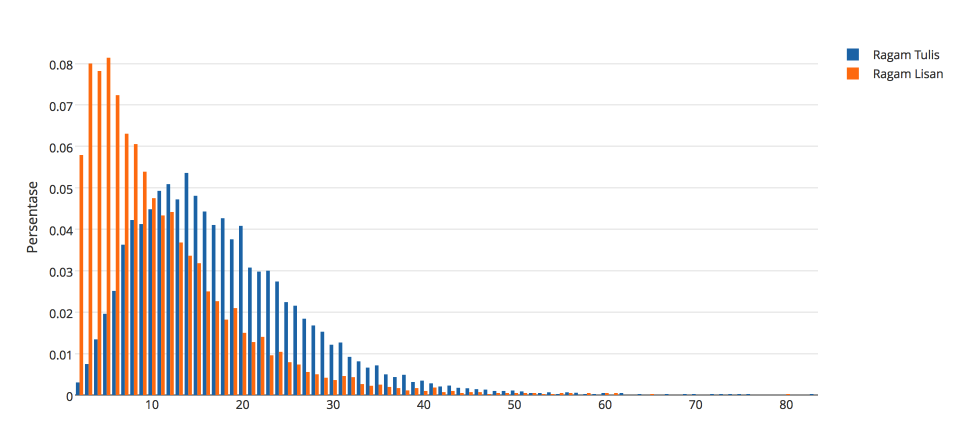
\includegraphics[width=1
	\textwidth] {pics/Jumlah_kata.png} 
	\caption{Diagram perbandingan jumlah konstituen data ragam lisan dan tulis} 
	\label{fig:jumlah_kata} 
\end{figure}

%%-----------------------------------------------------------------------------%
\section{Temuan 2: Pemusatan data ragam lisan pada klasifikasi kalimat pendek (\textless= 10 konstituen)}
%%-----------------------------------------------------------------------------%
Pemusatan data pada klasifikasi kalimat pendek (\textless= 10 konstituen) pada data ragam lisan cukup besar hingga melebihi 50\% dari total jumlah kalimat dalam korpus tersebut. Hal ini berdampak pada perbandingan rata-rata nilai DL serta MDD antara data ragam tulis dan lisan pada kelompok klasifikasi tersebut (\tab~\ref{tab:DL_MDD_pendek}).

\begin{center}
 \label{table:DL_MDD_pendek}
 \caption{Perbandingan rata-rata nilai DL dan MDD pada klasifikasi kalimat pendek}
  \begin{tabular}{ | l | l |}
    \hline
    \hline
  \end{tabular}
\end{center}

Berdasarkan \tab~\ref{tab:perbandingan_DL_MDD}, Nilai DL dan MDD data ragam lisan lebih kecil dibandingkan data ragam tulis pada klasifikasi kalimat pendek. Berbeda dengan temuan tanpa memperhitungkan klasifikasi panjang kalimat, Terutama pada nilai DL yang bersifat cukup linier terhadap panjang kalimat, rata-rata nilai DL pada data ragam lisan (8,76) menjadi lebih rendah karena pemusatan data dengan jumlah konstituen yang mendekati minimum dibandingkan dengan data ragam tulis yang nilai tertingginya berada pada kelompok klasifikasi kalimat menengah. Pada kelompok klasifikasi ini, rata-rata nilai MDD data ragam lisan juga lebih kecil dibandingkan data ragam tulis. Berdasarkan temuan ini, dapat diasumsikan bahwa penggunaan kalimat pendek mungkin digunakan menjadi salah satu strategi dalam percakapan lisan untuk meningkatkan efisiensi. Dalam beberapa kasus di korpus data ragam lisan, ditemukan ujaran-ujaran yang sebenarnya merupakan klausa yang lepas dari klausa pada ujaran sebelumnya. Ujaran-ujaran ini banyak ditemukan diawali dengan konjungsi "dan" pada posisi pertama dalam ujaran. 

%%-----------------------------------------------------------------------------%
\subsection{Temuan 3: Perbandingan nilai DL dan MDD antara data ragam tulis dan lisan pada klasifikasi kalimat menengah (11-20 konstituen)}
%%-----------------------------------------------------------------------------%
Pada kelompok klasifikasi kalimat menengah (11-20 konstituen), terlihat adanya perbbandingan terbalik antara rata-rata nilai DL dan MDD pada kedua korpus data (\tab~\ref{tab:DL_MDD_menengah}). Untuk nilai DL, data ragam lisan memiliki rata-rata yang sedikit lebih rendah (33,05) dibandingkan data ragam tulis (33,32). Perbedaan ini diakibatkan oleh pemusatan ujaran ragam lisan yang banyak mendekati kalimat pendek, sedangkan persebaran ujaran ragam tulis di kelompok klasifikasi ini cukup merata. Meskipun begitu, temuan yang menarik adalah bahwa rata-rata nilai MDD data ragam tulis (2,31) lebih rendah dibandingkan dengan data ragam lisan (2,41). 

\begin{center}
 \label{table:DL_MDD_menengah}
 \caption{Perbandingan rata-rata nilai DL dan MDD pada klasifikasi kalimat menengah}
  \begin{tabular}{ | l | l |}
    \hline
    \hline
  \end{tabular}
\end{center}

Rata-rata nilai DL dan MDD kedua korpus data yang berbanding terbalik menunjukkan adanya indikasi bahwa pada panjang kalimat tertentu, jumlah konstituen yang lebih sedikit tidak selalu berfungsi sebagai strategi untuk menghasilkan kalimat yang efisien dari segi dependensi. Indikasi pada kelompok klasifikasi ini menarik karena memperlihatkan bahwa meskipun jumlah nilai yang dihasilkan semua tautan dependensi lebih kecil, tidak berarti menggambarkan jarak antarkonstituen yang lebih kecil juga.

%%-----------------------------------------------------------------------------%
\subsection{Temuan 4: Perbandingan struktur ujaran data ragam tulis dan lisan pada klasifikasi kalimat panjang (\textgreater20 konstituen) terkait nilai DL dan MDD}
%%-----------------------------------------------------------------------------%

Berbeda dengan kedua klasifikasi kalimat sebelumnya, rata-rata nilai DL dan MDD pada data ragam tulis lebih kecil dibandingkan data ragam lisan (\tab~\ref{tab:DL_MDD_panjang}). Hal ini berarti terlepas dari persebaran ujarannya yang cukup banyak (31,13\% dari keseluruhan korpus data ragam tulis), ujaran dengan jumlah konstituen yang lebih banyak data ragam tulis cenderung memiliki struktur yang lebih efisien dibandingkan dengan data ragam lisan. Pada kelompok klasifikasi menengah, nilai MDD data ragam tulis lebih kecil dibandingkan data ragam lisan. Temuan tersebut dan temuan pada klasifikasi ini menunjukkan bahwa mulai panjang kalimat tertentu, meskipun kompleksitas kalimat semakin tinggi (nilai DL makin tinggi), data ragam tulis menunjukkan struktur yang menyebabkan tautan antarkonstituen lebih pendek sehingga mendukung efisiensi ujaran.

\begin{center}
 \label{table:DL_MDD_panjang}
 \caption{Perbandingan rata-rata nilai DL dan MDD pada klasifikasi kalimat panjang}
  \begin{tabular}{ | l | l |}
    \hline
    \hline
  \end{tabular}
\end{center}

Untuk memberikan ilustrasi terhadap perbandingan struktur ujaran kelompok klasifikasi kalimat panjang, berikut adalah beberapa contoh ujaran dengan jumlah konstituen sebanyak 31 yang diambil dari kedua korpus data (\pic~\ref{fig:}, \pic~\ref{fig:},\pic~\ref{fig:},\pic~\ref{fig:}, dan \pic~\ref{fig:}). Kelima ujaran pada \pic~\ref{fig:}, \pic~\ref{fig:},\pic~\ref{fig:},\pic~\ref{fig:}, dan \pic~\ref{fig:} menunjukkan adanya karakter utama yang membedakan struktur ujaran pada data ragam tulis dan lisan. Kata "penting" pada kalimat T31a dan "ditingkatkan" pada kalimat T31b merupakan konstituen induk dari keseluruhan kalimat (root) yang memiliki beberapa tautan dependensi terhadap konstituen terikatnya. Kesamaan kedua kalimat ini adalah bahwa konstituen induk (head) berikutnya yang diikat oleh root cenderung memiliki jumlah konstituen sedikit meskipun mengandung beberapa klausa terikat. Head berikutnya ini juga sama-sama mengikat head lain pada kalimat. 

Pada kalimat T31a, "penting" mengikat "memperbaiki" yang dihubungkan dengan konjungsi tujuan "untuk". Sedangkan pada kalimat T31b, "ditingkatkan" mengikat "mempercepat" yang juga dihubungkan dengan konjungsi tujuan "untuk". Pada kedua kalimat, head ketiga, keempat, dan seterusnya tidak memiliki tautan langsung dengan root, melainkan memiliki hubungan secara berlanjut. Hubungan ini membentuk lapisan level dependensi yang semakin mendalam. Dalam diagram pohon kedua ujaran, hubungan ini terlihat melalui pergerakan simpai dan percabangan yang semakin menurun ke arah sesudah root (kanan). Percabangan menurun ke kanan ini menunjukkan indikasi adanya strategi untuk menghasilkan dependensi positif (konstituen terikat sesudah konstituen induk) dan hubungan klausa yang bersifat berlanjut (seri) seiring berjalannya ujaran. Hal ini berarti untuk percabangan setelah root dapat langsung diproses oleh kognisi manusia karena root sudah direalisasikan terlebih dahulu (Tesniere, 1959; Wang & Liu, 2017). \todo{Kalimat T31a memiliki nilai DL XX dan nilai MDD XX, sedangkan kalimat T31b memiliki nilai DL XX dan nilai MDD XX}

\begin{figure}
	\centering 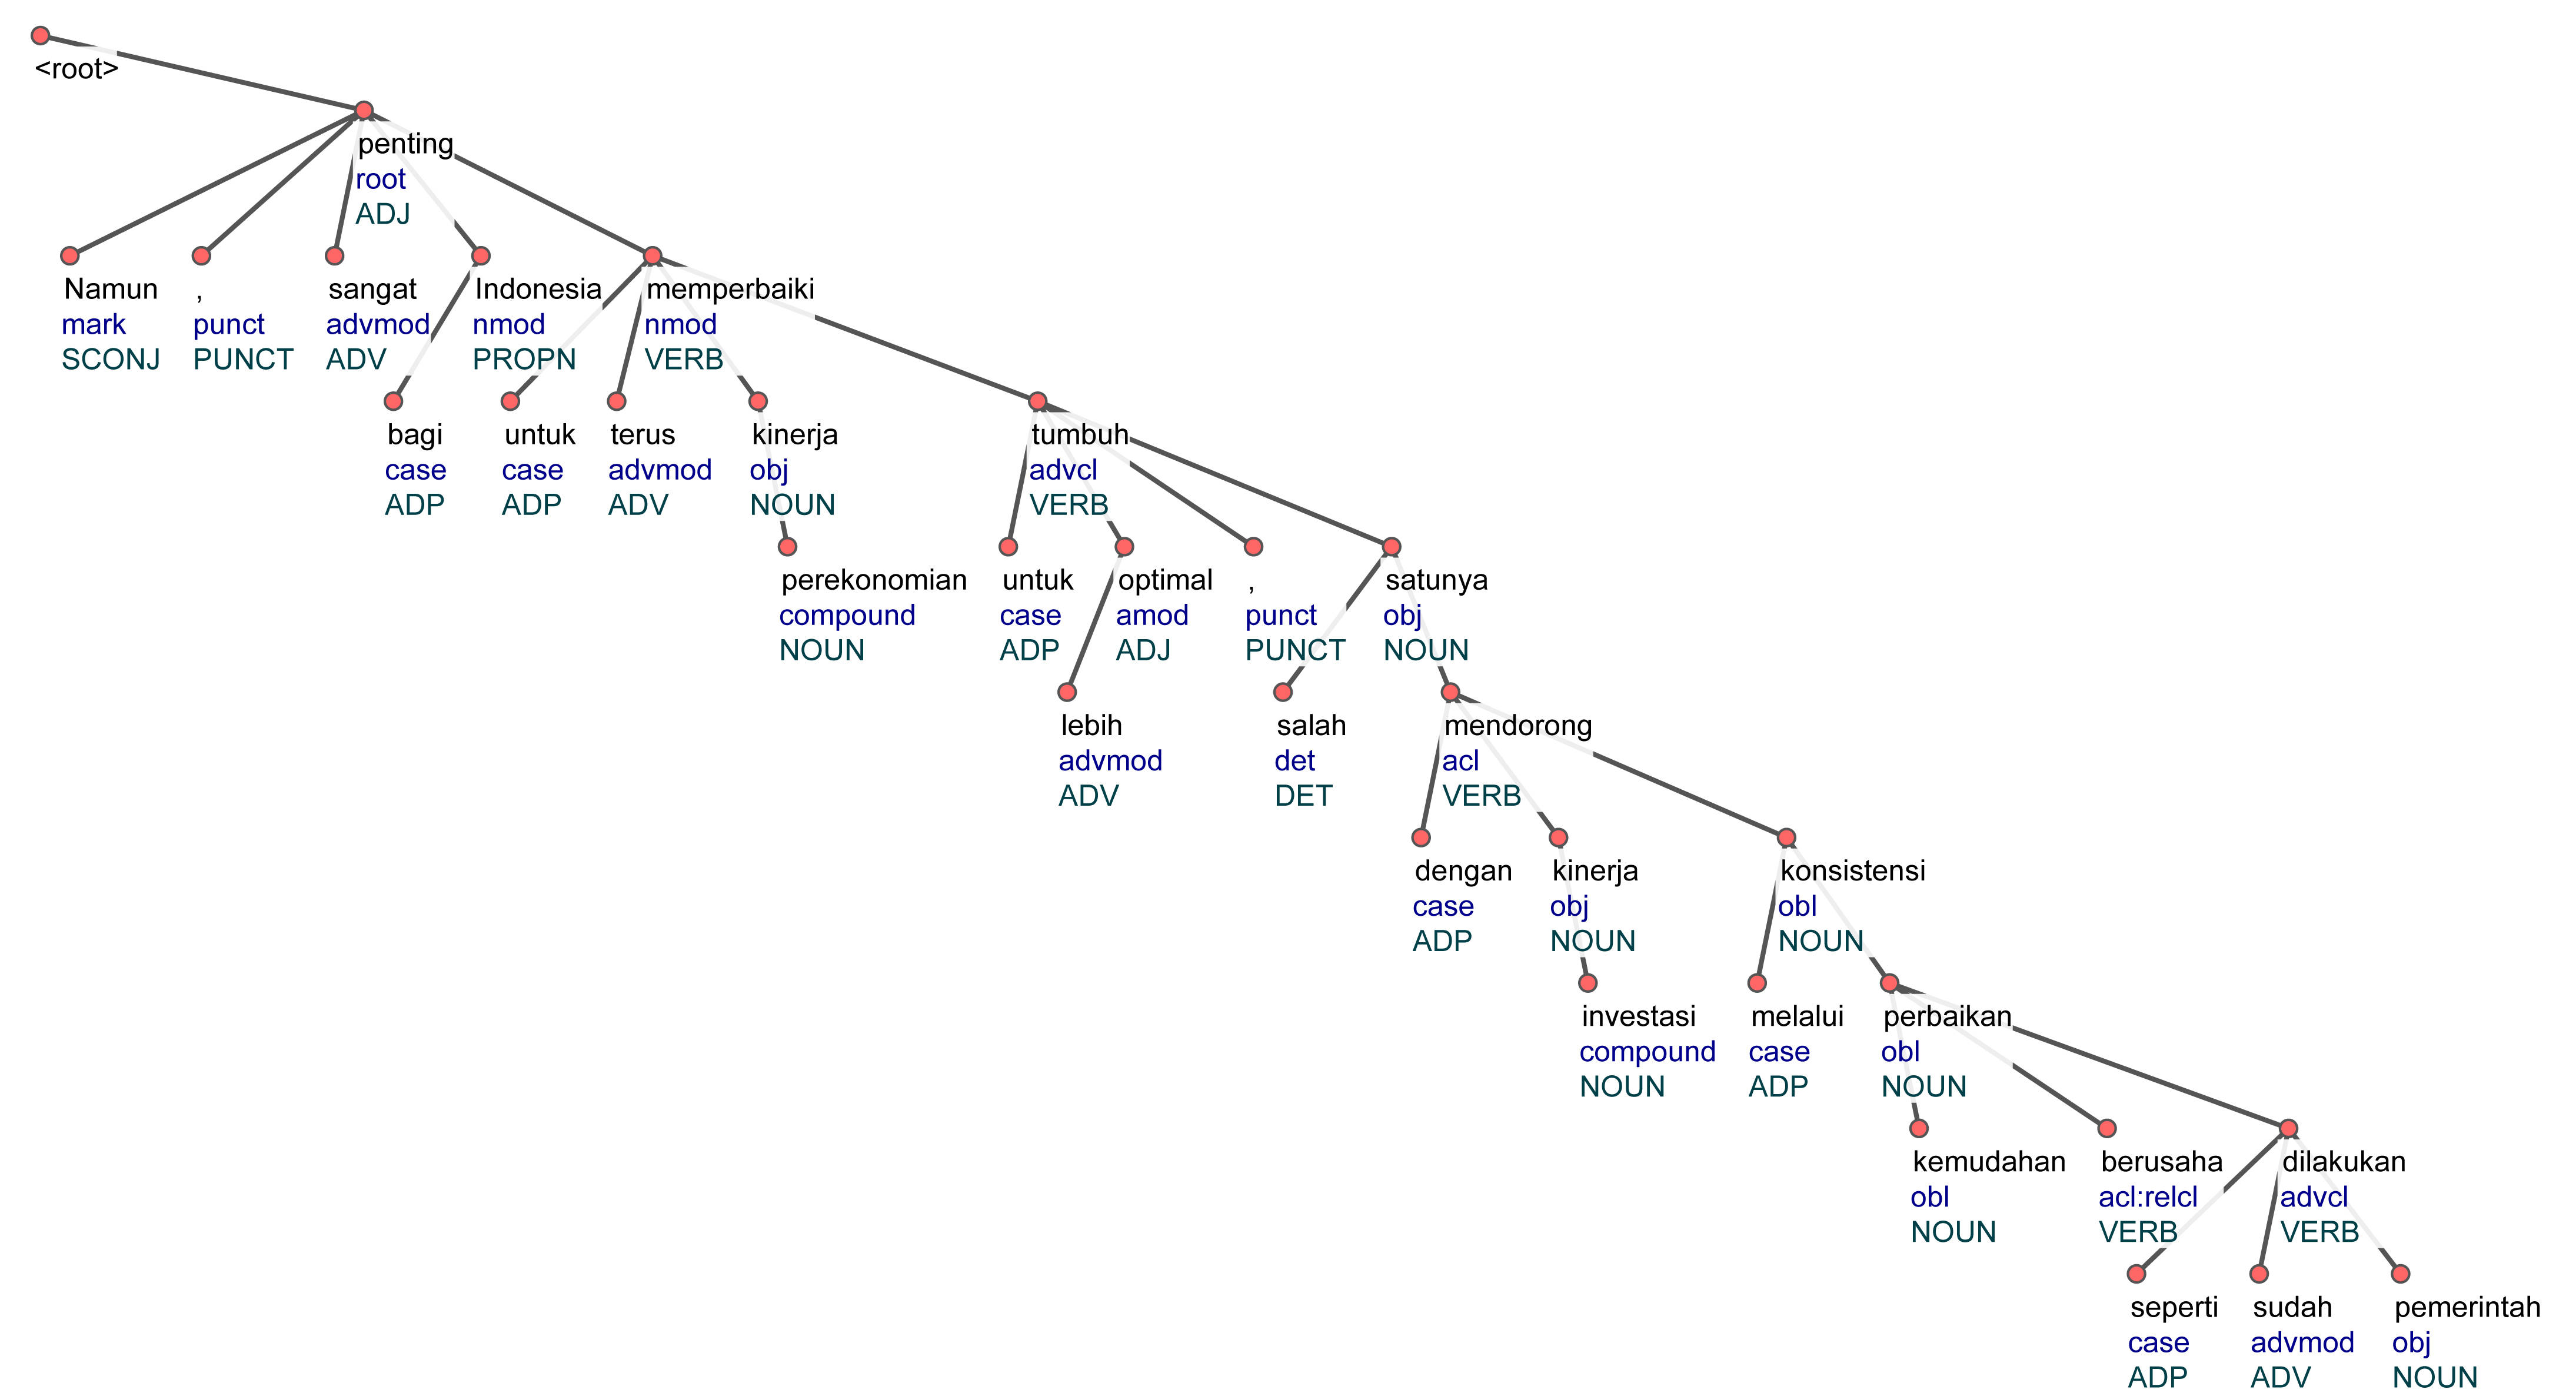
\includegraphics[width=1
	\textwidth] {pics/ts2079.jpg} 
	\caption{Kalimat T31a pada data ragam tulis} 
	\label{fig:ts2079} 
\end{figure}

\begin{figure}
	\centering 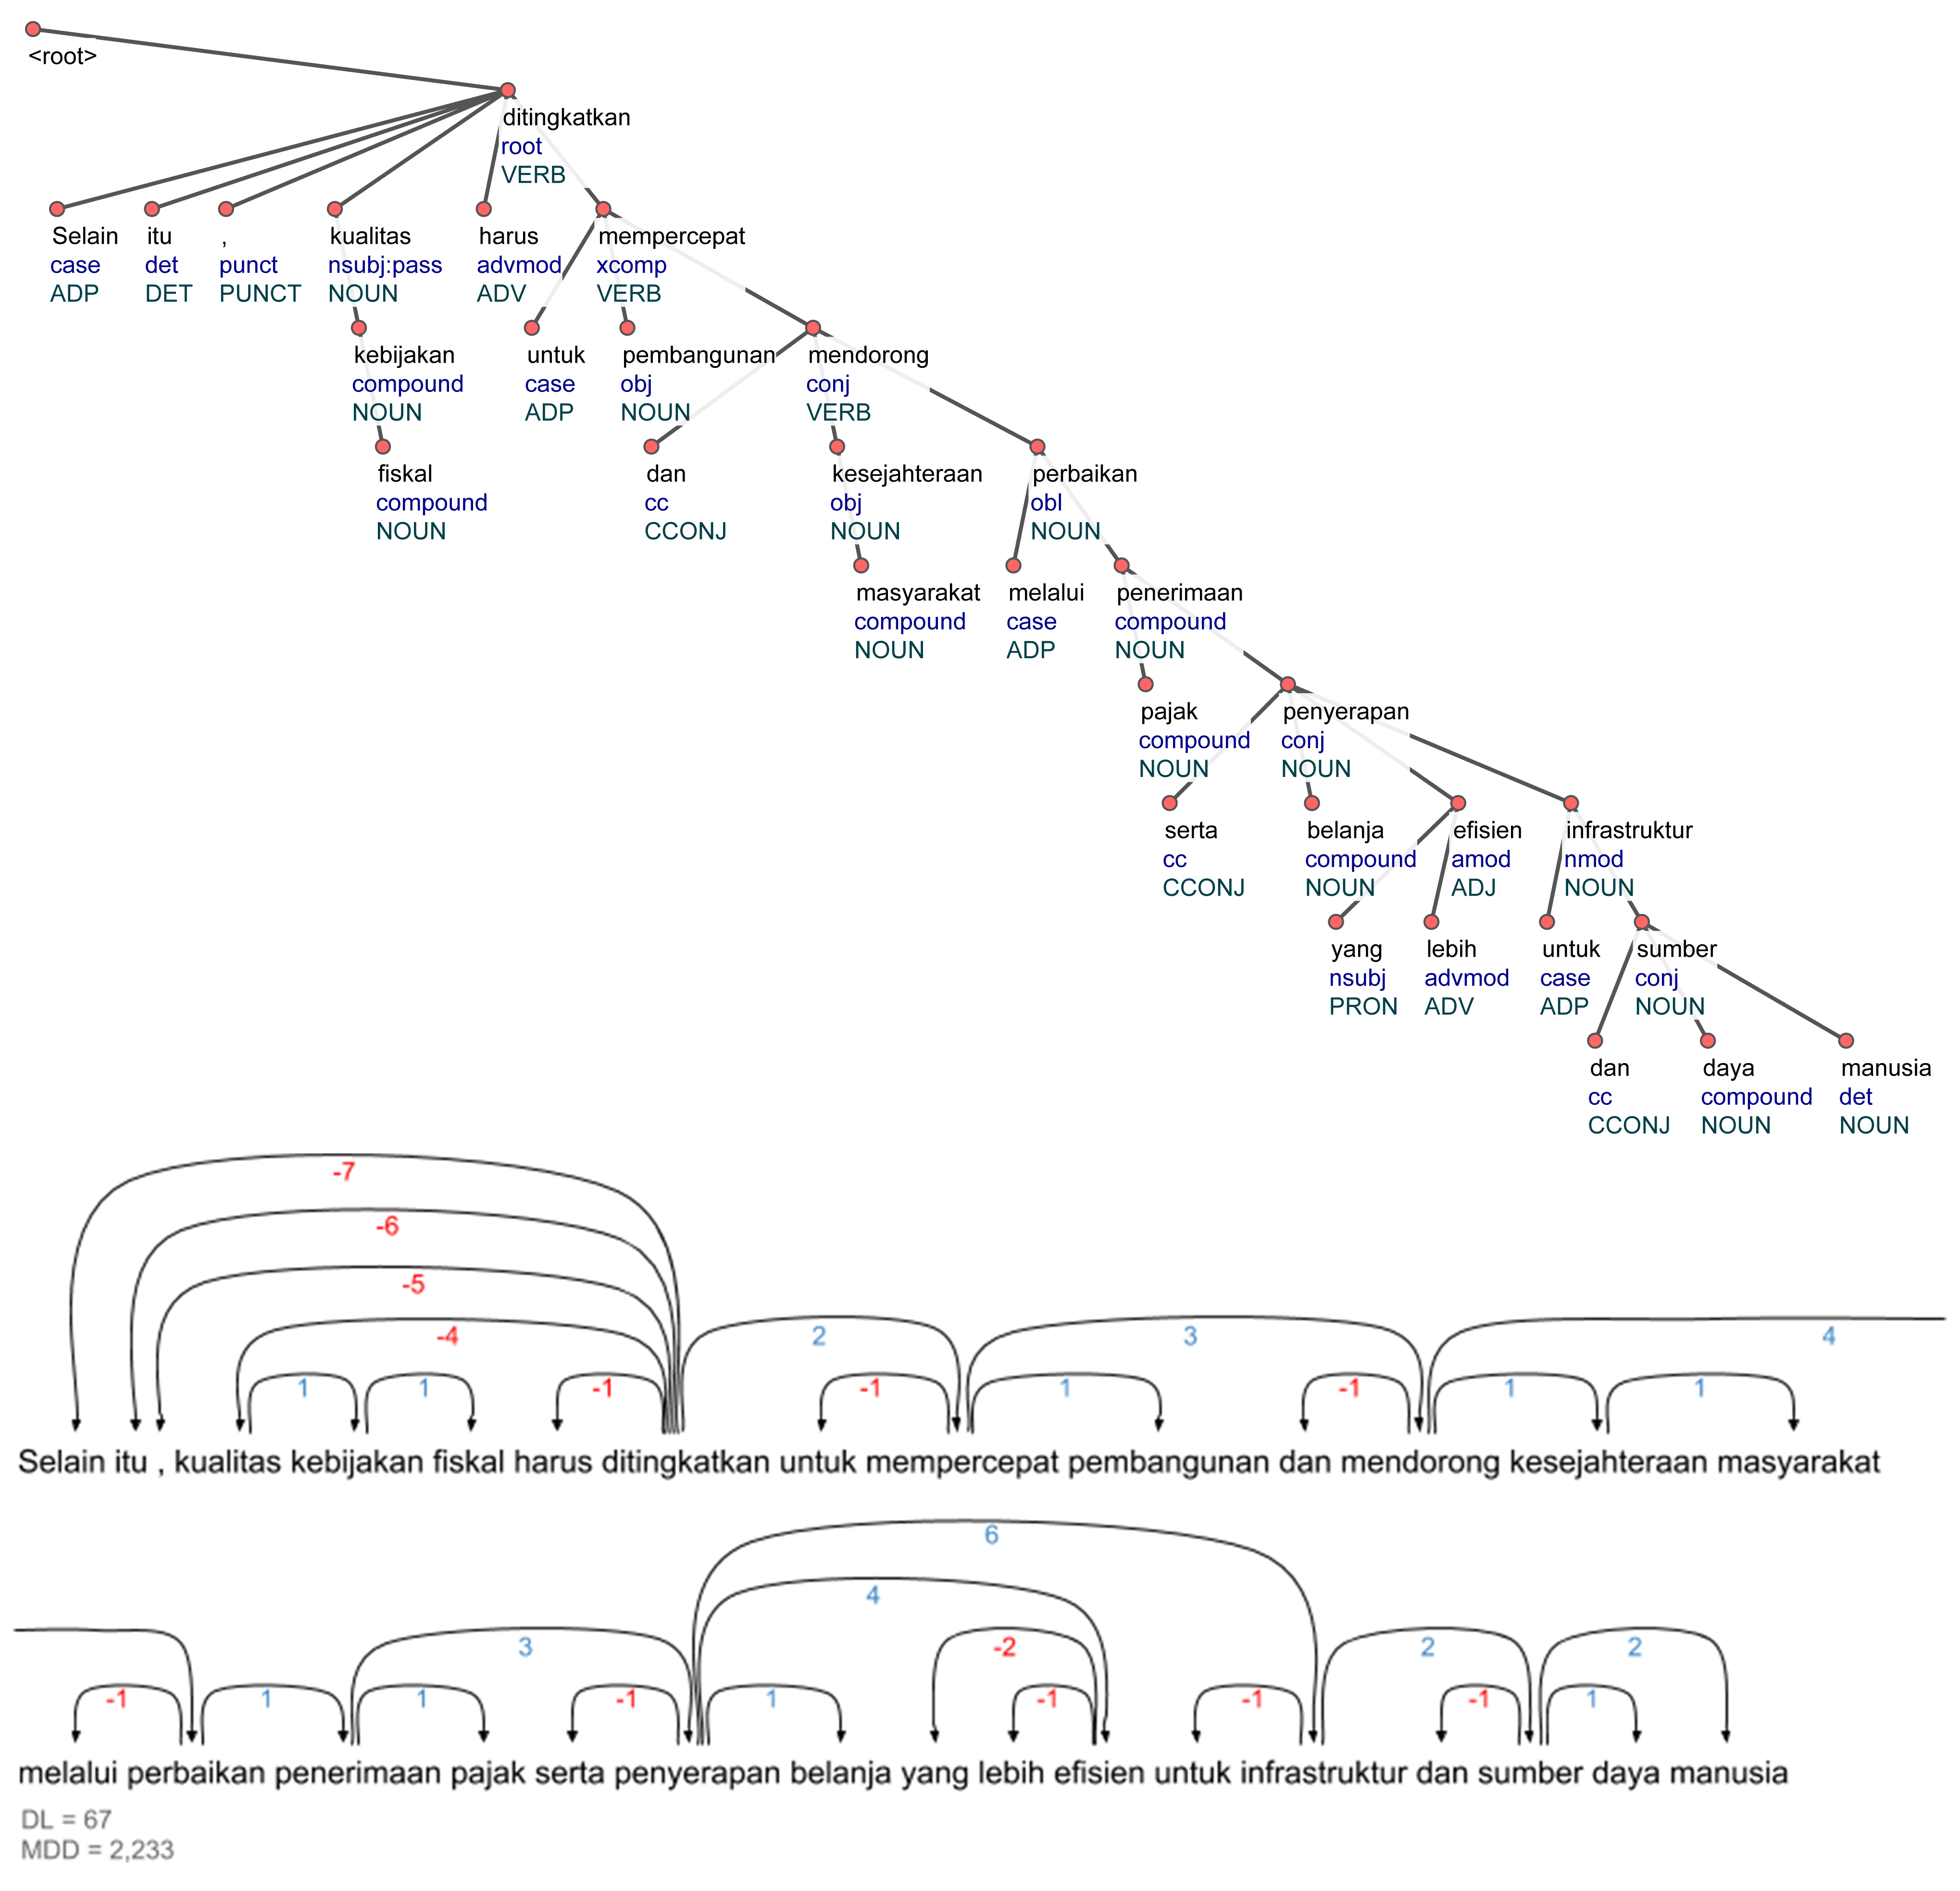
\includegraphics[width=1
	\textwidth] {pics/ts2081.jpg} 
	\caption{Kalimat T31b pada data ragam tulis} 
	\label{fig:ts2081} 
\end{figure}

Kalimat L31a, L31b, dan L31c sedikit berbeda satu sama lain namun memiliki karakter utama yang serupa yang membedakannya dengan data ragam tulis. Salah satunya adalah perbedaan posisi root L31a, L31b, dan L31c. Posisi klausa tempat root L31a berada  terletak di awal ujaran, sedangkan root L31b terletak di tengah, dan root L31c terletak di akhir. Persebaran letak root ini jarang ditemukan pada klasifikasi kalimat panjang dalam korpus data ragam tulis. Berdasarkan diagram pohon ujaran L31a, L31b, dan L31c, perbedaan yang paling terlihat dibandingkan dengan diagram pohon T31a dan T31b adalah percabangannya yang bersifat menyebar dan bukan semakin menurun ke satu arah tertentu. Pada ujaran L31a, terdapat 2 percabangan utama dengan root "berdatangan" dan "dipaksa". Kedua percabangan tersebut memiliki klausa-klausa di dalamnya yang dapat mengandung klausa lain. Percabangan serupa juga ditemui pada L31b (tautan antara "menanyakan" dengan "memastikan" dan "menanyakan" dengan "dibantah") dan L31c (tautan antara "kira" dengan "hemat", "kira" dengan "Pak", dan "kira" dengan "salah"). 

\begin{figure}
	\centering 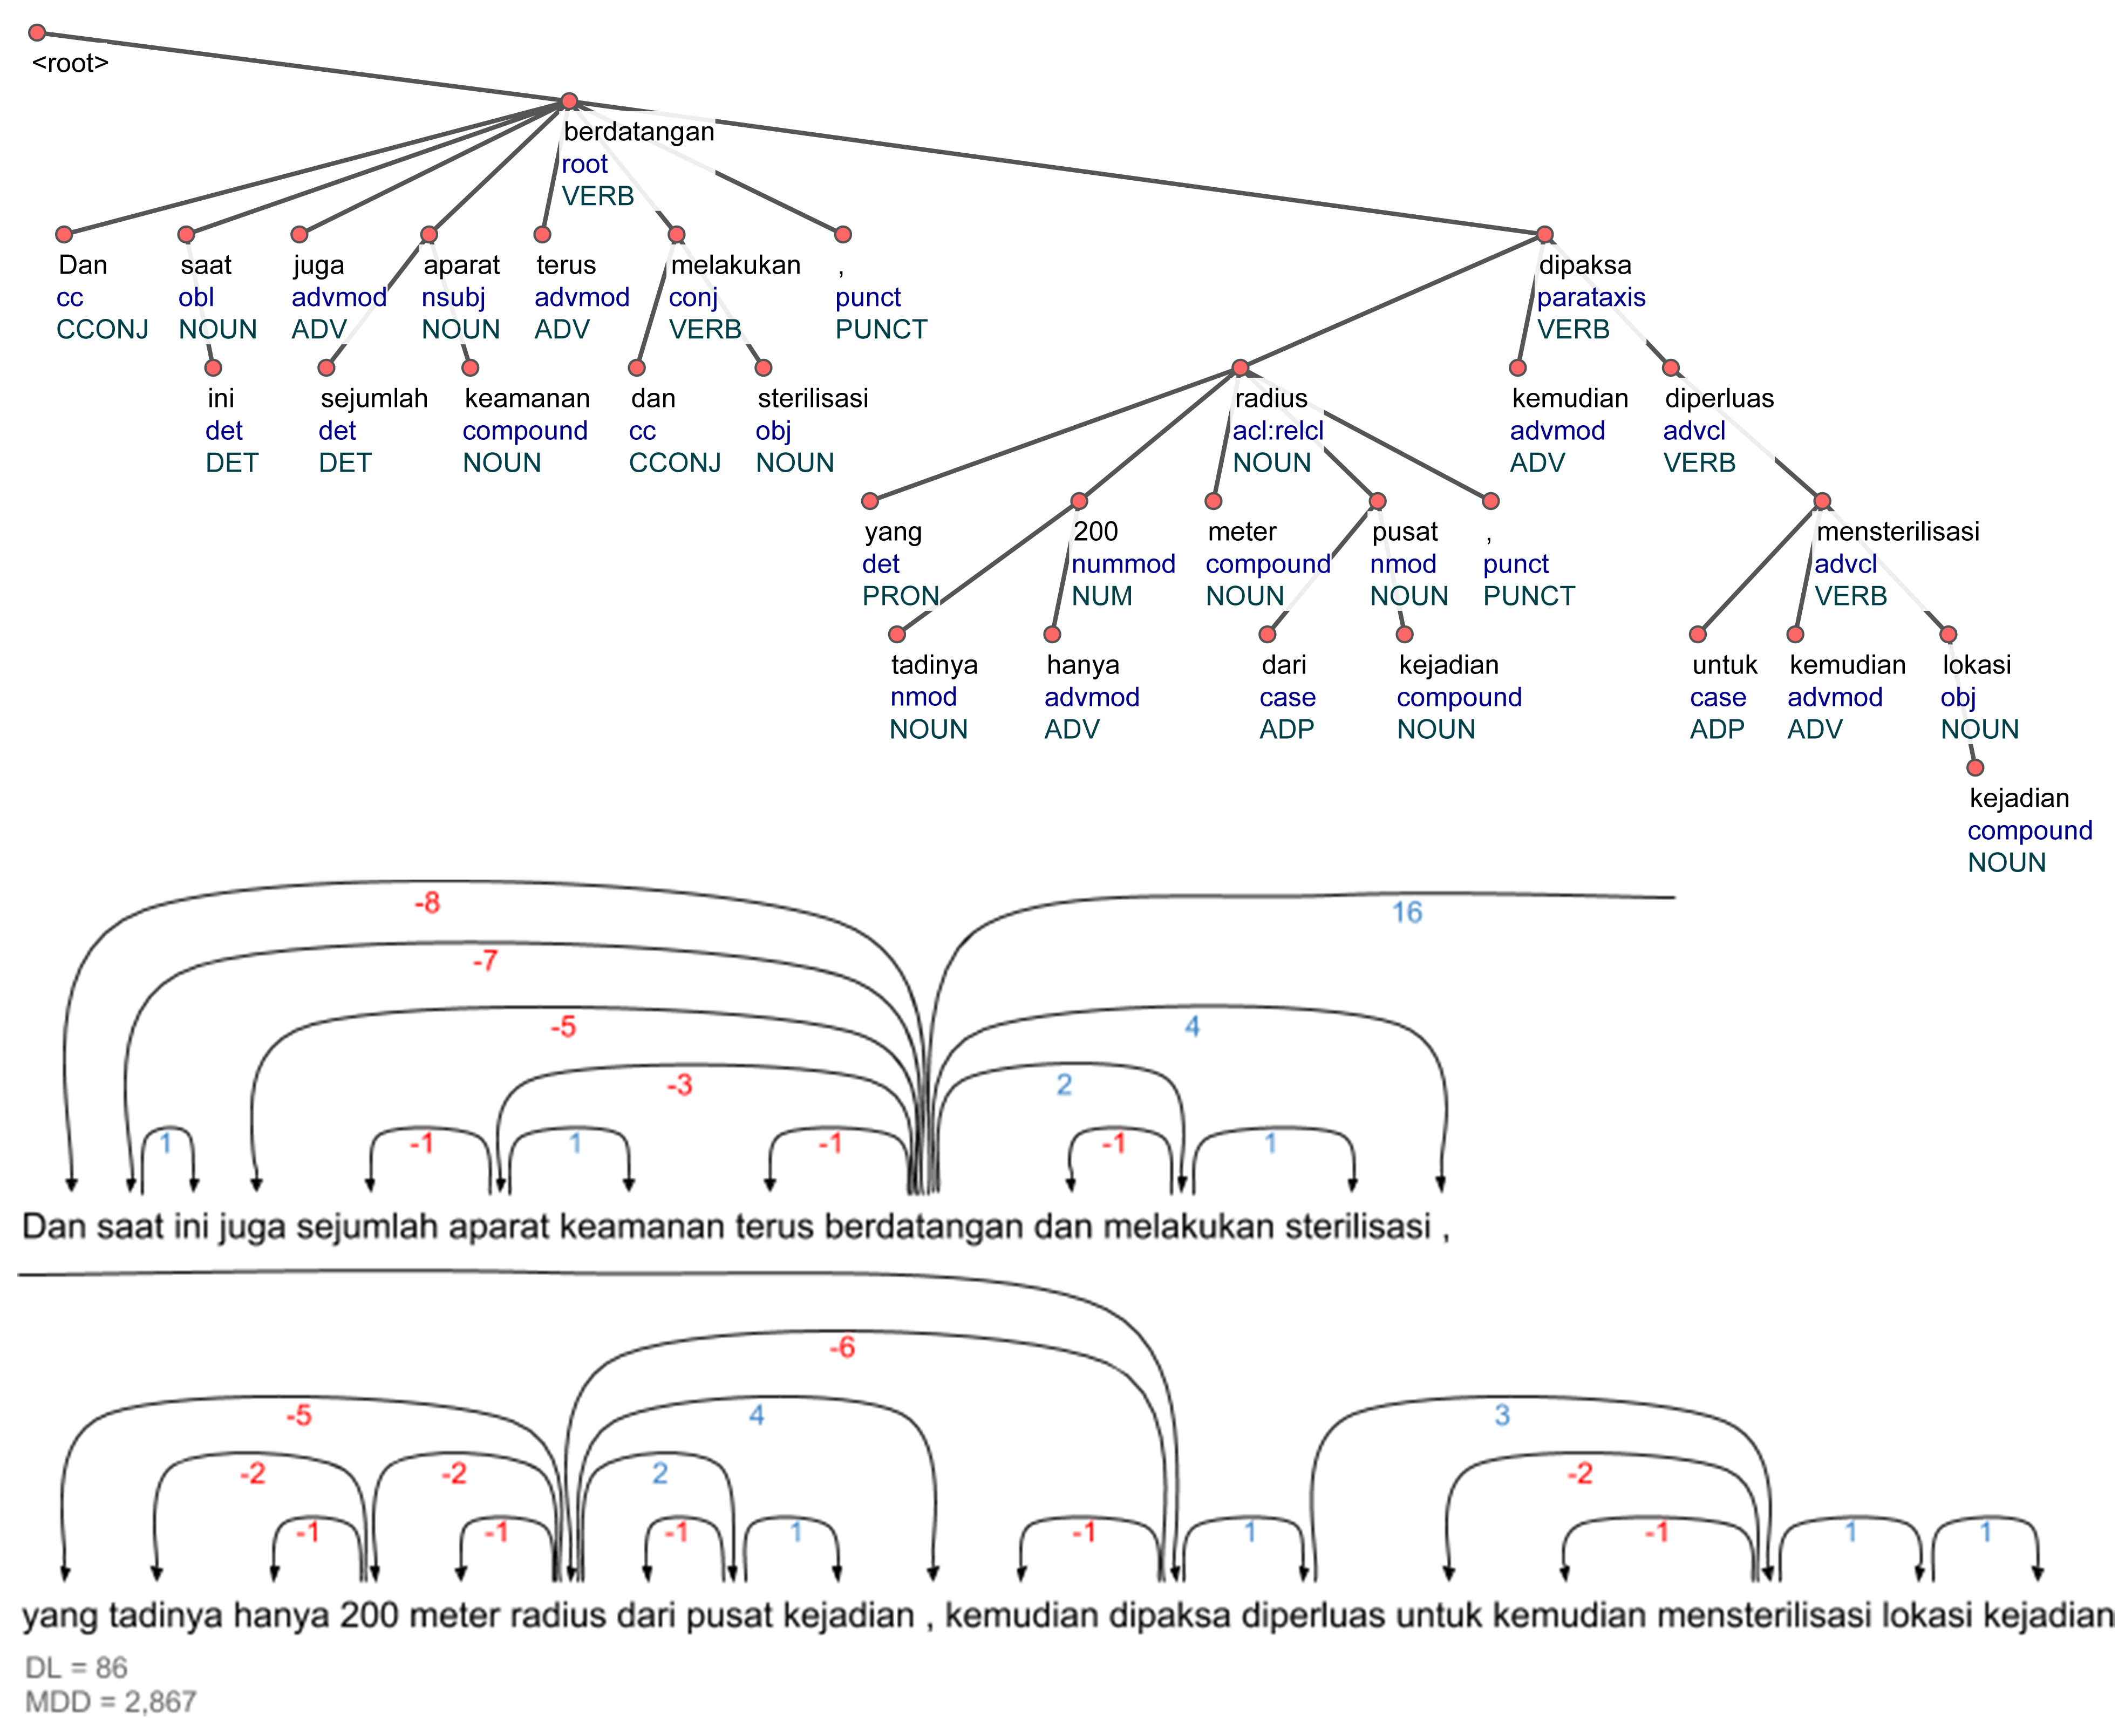
\includegraphics[width=1
	\textwidth] {pics/ls1716.jpg} 
	\caption{Kalimat L31a pada data ragam lisan} 
	\label{fig:ls1716} 
\end{figure}

\begin{figure}
	\centering 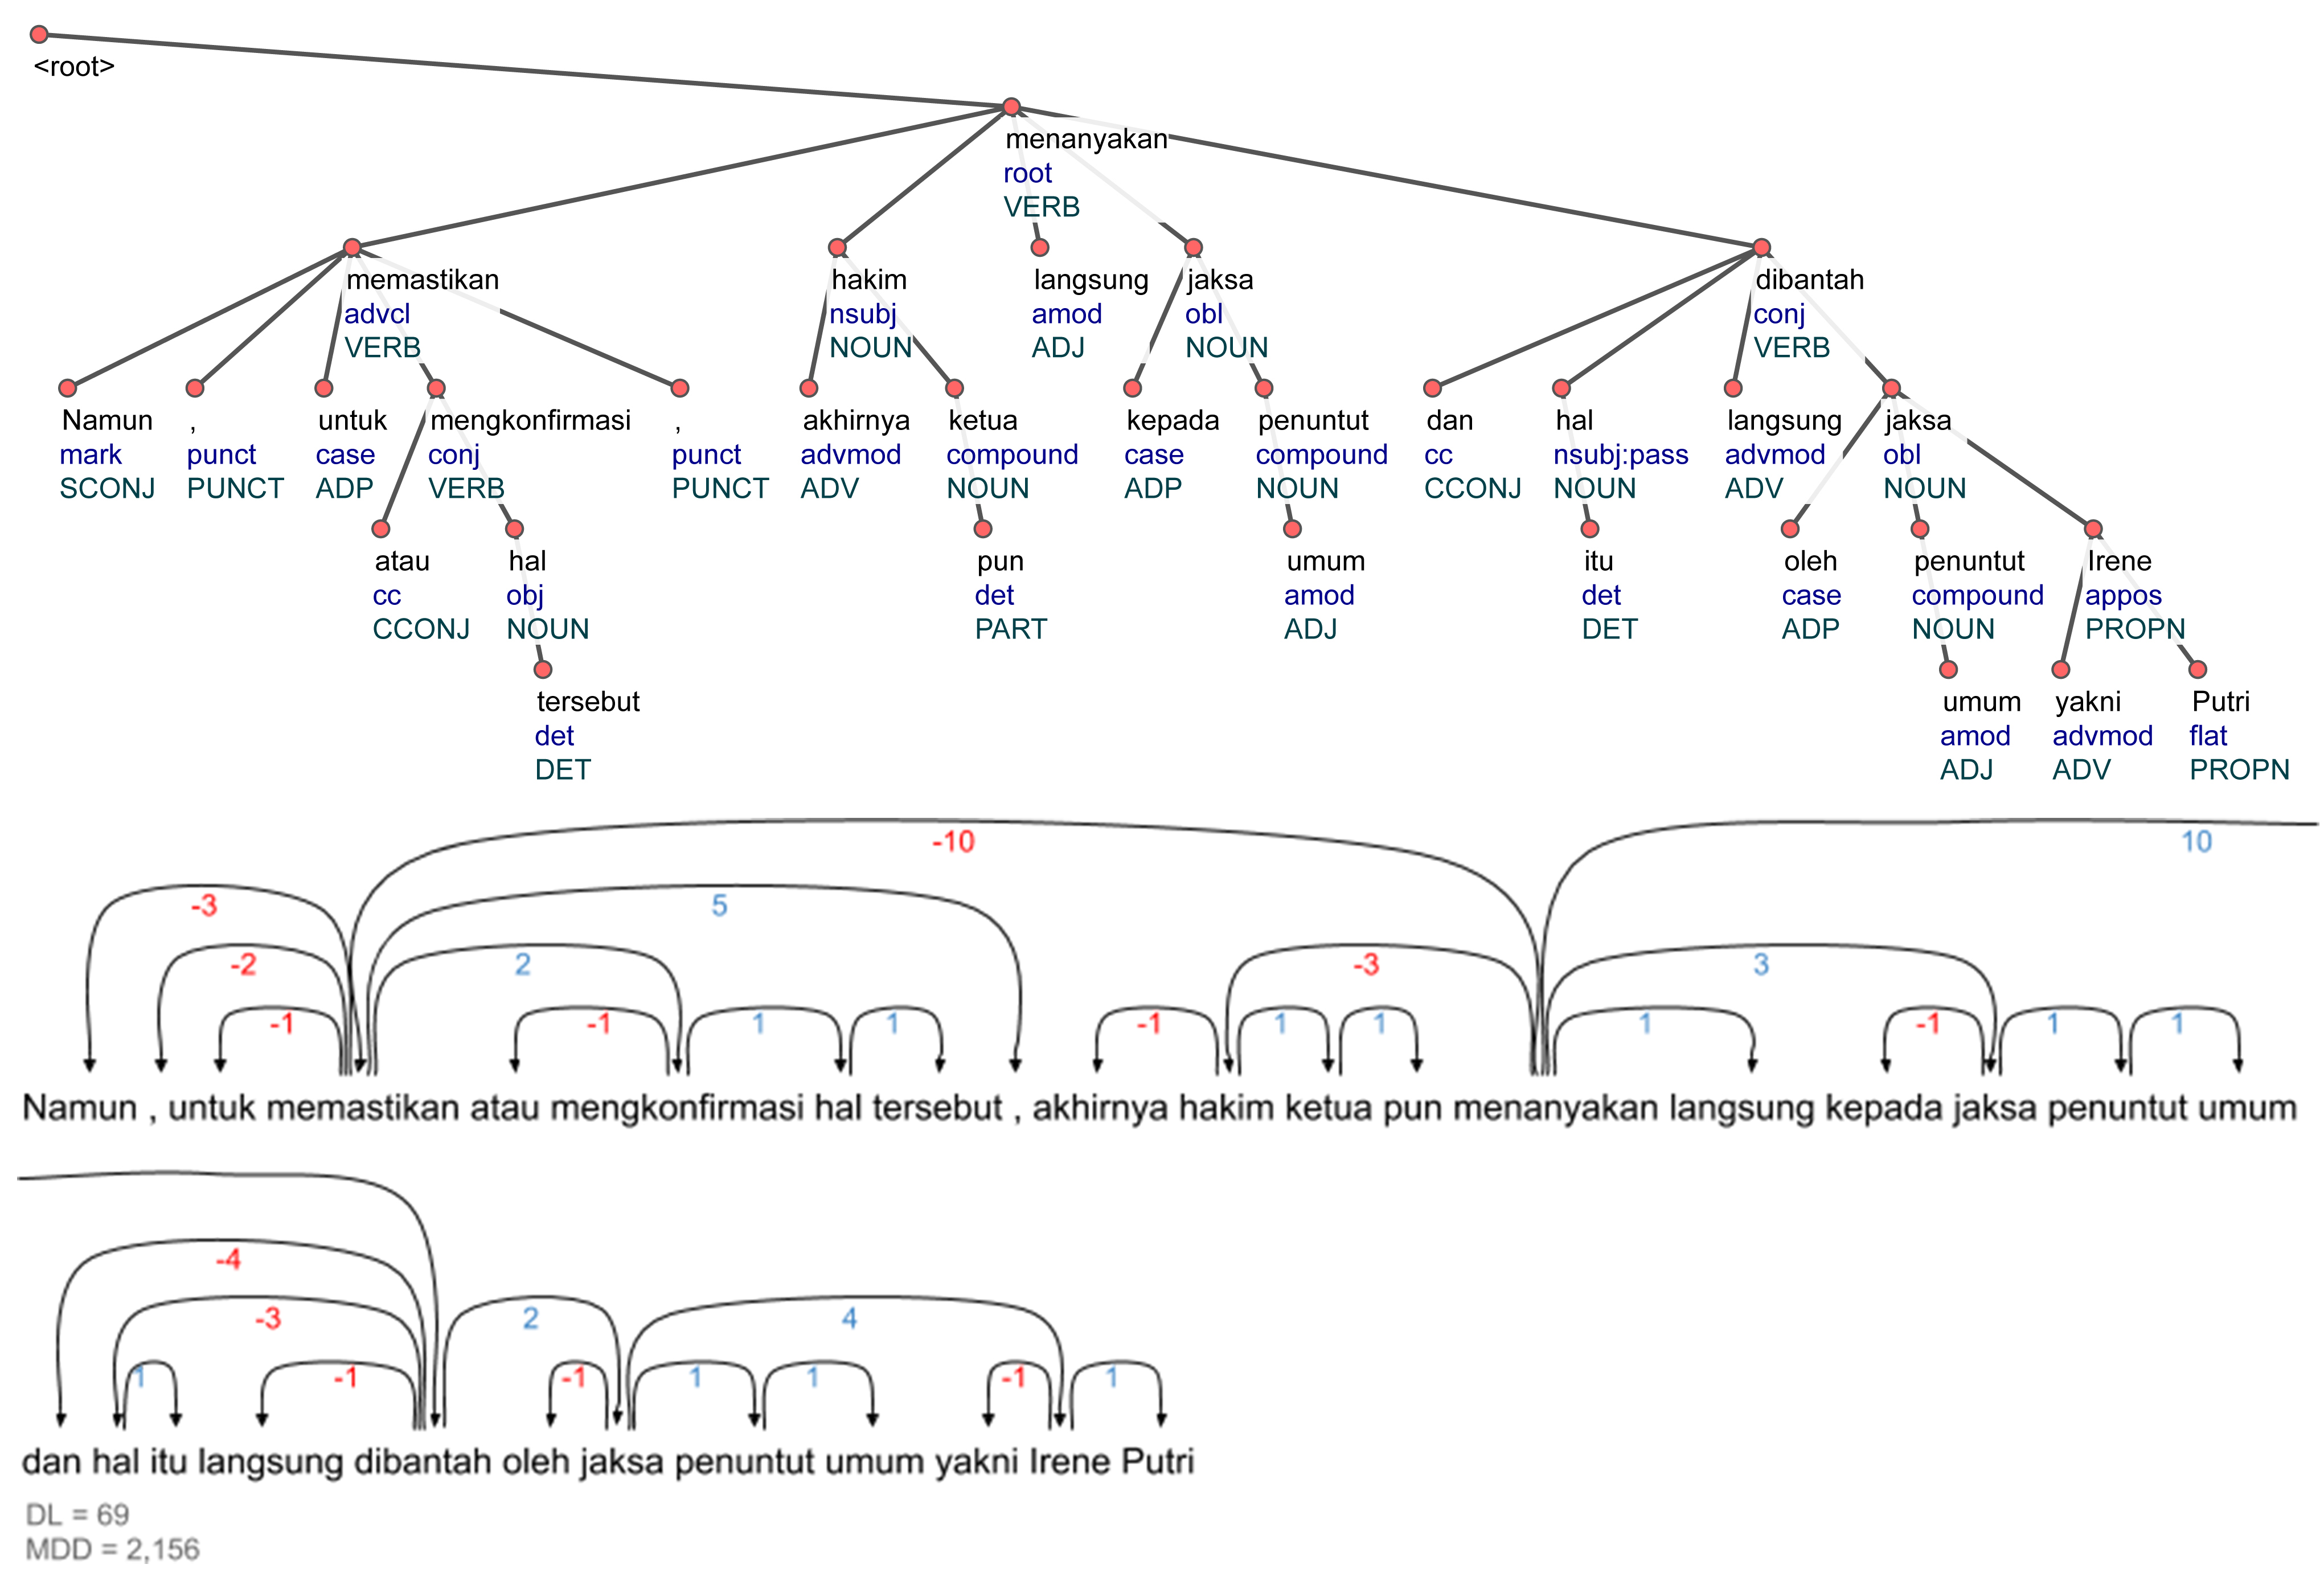
\includegraphics[width=1
	\textwidth] {pics/ls16.jpg} 
	\caption{Kalimat L31b pada data ragam lisan}
	\label{fig:ls16} 
\end{figure}

\begin{figure}
	\centering 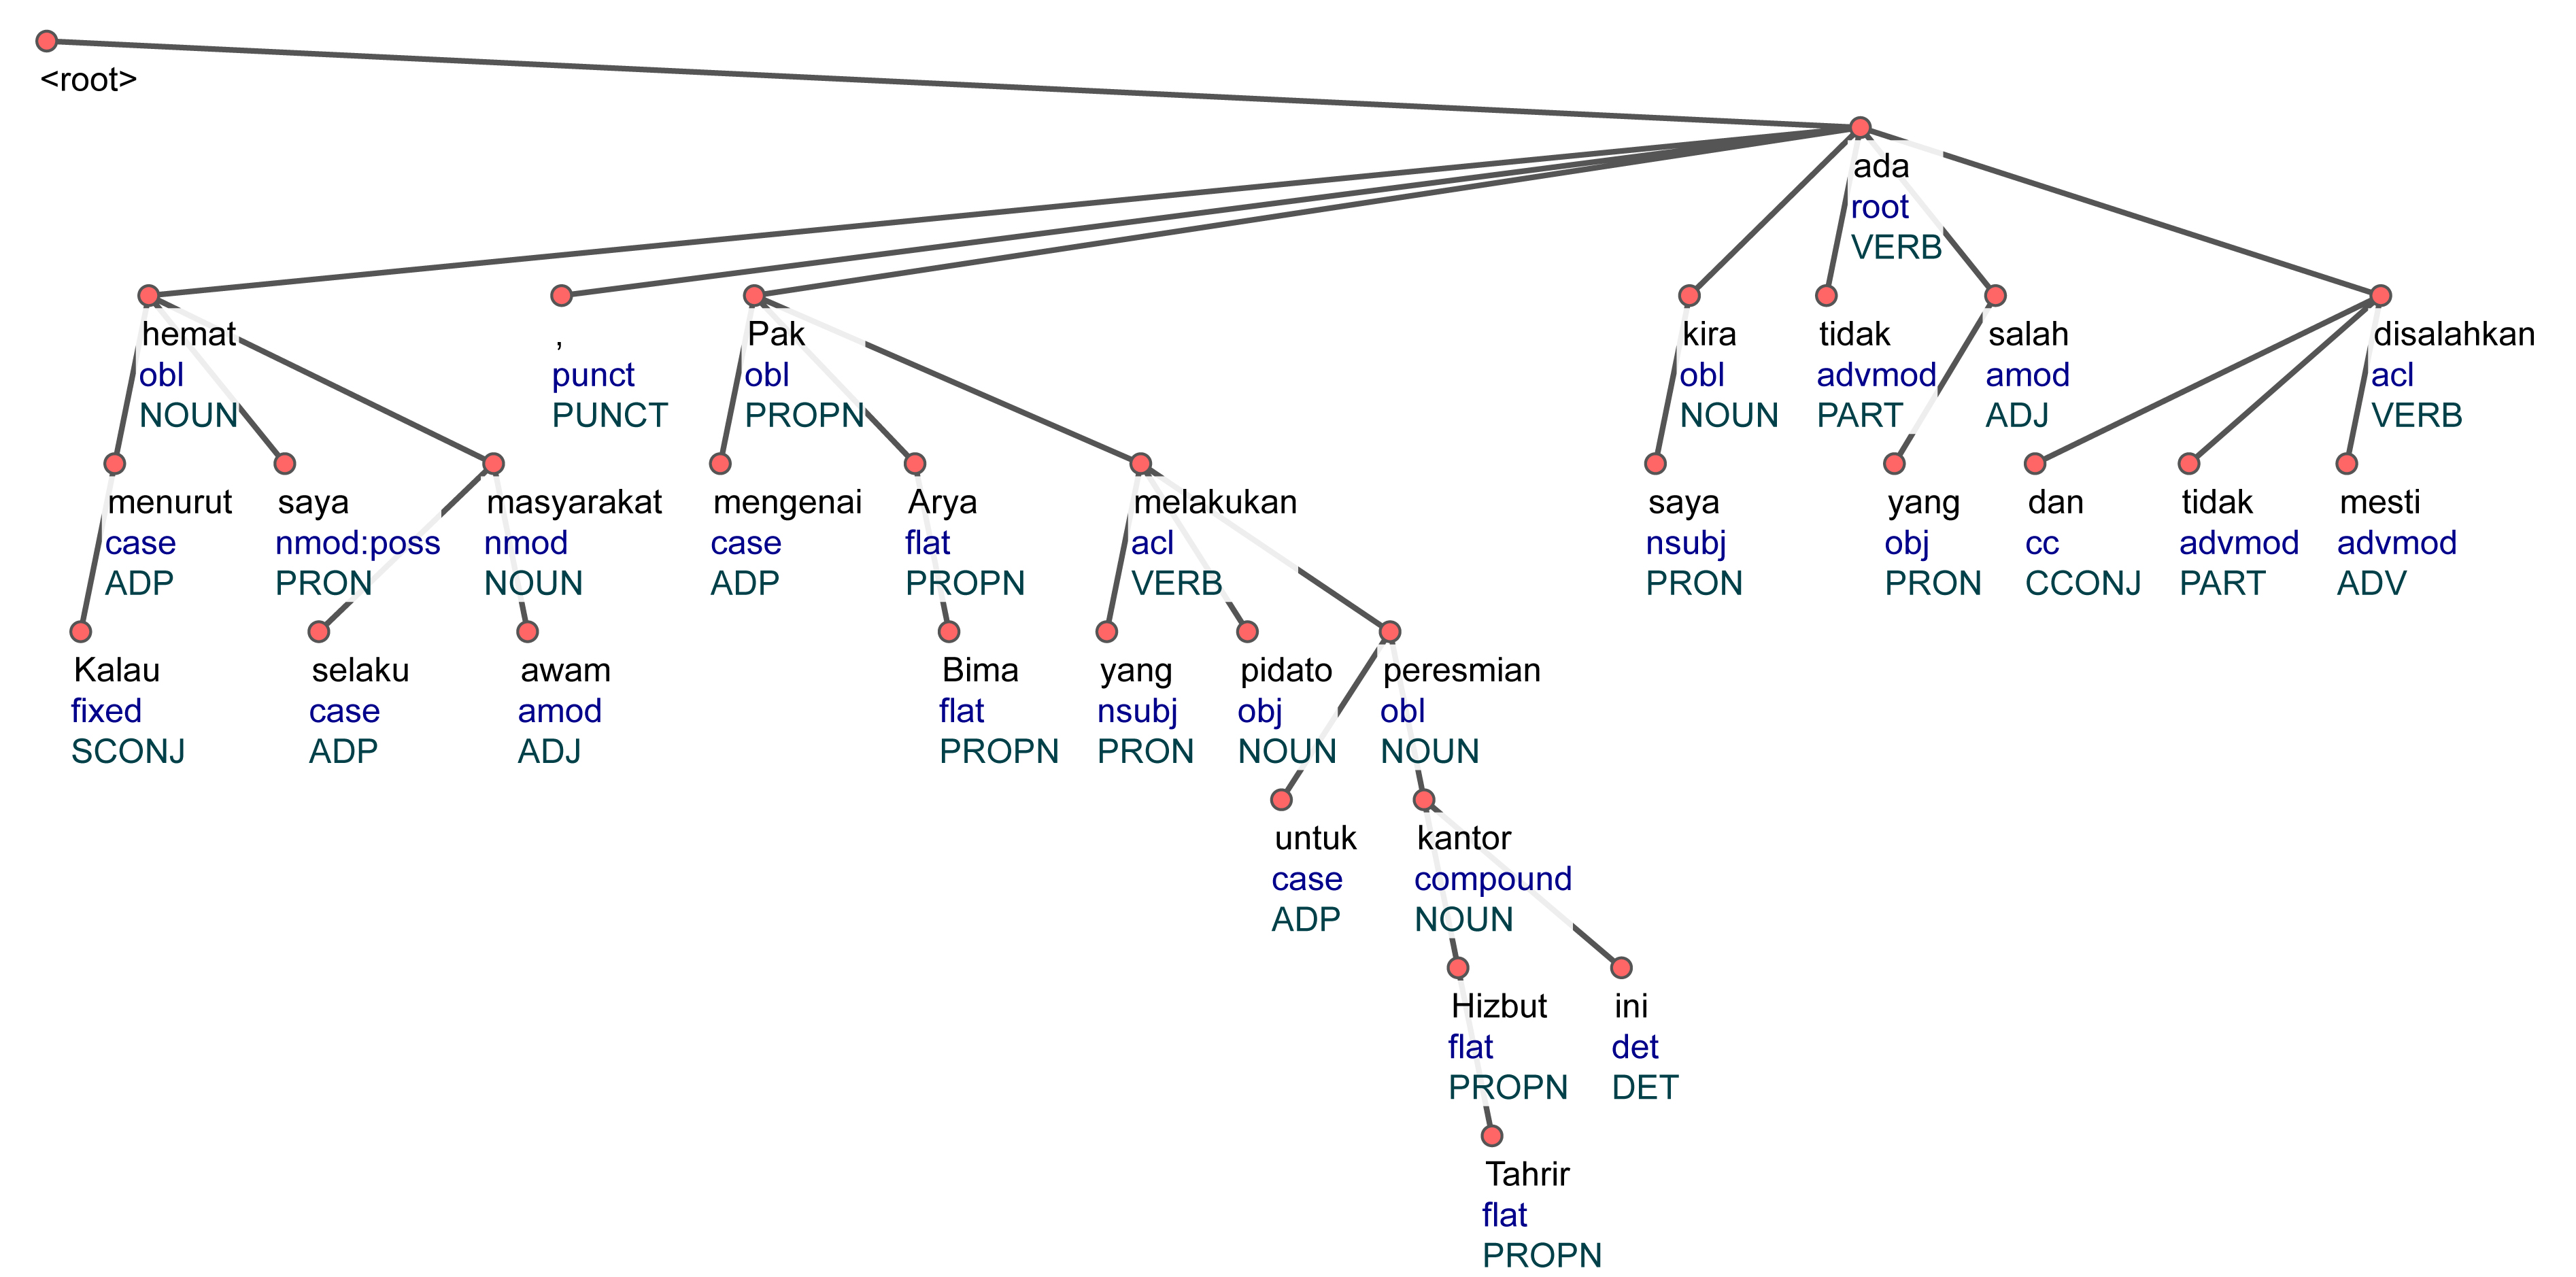
\includegraphics[width=1
	\textwidth] {pics/ls114.jpg} 
	\caption{Kalimat L31c pada data ragam lisan}
	\label{fig:ls114} 
\end{figure}

Percabangan utama yang tersebar secara cukup merata pada ketiga ujaran tersebut menunjukkan indikasi hubungan klausa yang tidak bersifat berlanjut, namun paralel. L31b dan L31c memiliki percabangan utama sebelum root sehingga secara kolaktif membentuk dependensi utama yang negatif. Hal ini berarti seluruh informasi yang dibawa oleh klausa-klausa pada simpai dan percabangan sebelum root harus disimpan dalam memori kerja dan menunggu realisasi root agar penggalan informasi yang dibawa simpai tersebut dapat diproses secara utuh oleh kognisi manusia (Hawkins, 2014).

%%-----------------------------------------------------------------------------%
\section{Diskusi Temuan 2, 3, dan 4}
%%-----------------------------------------------------------------------------%
Berdasarkan percobaan acak yang dilakukan, analisis selanjutnya adalah melihat aspek-aspek yang mungkin mempengaruhi struktur ujaran sehingga memungkinkan terjadinya DLM dan DDM. Secara garis besar, analisis-analisis lanjutan untuk melihat aspek-aspek ini menghasilkan temuan strategi yang berkaitan dengan panjang kalimat, pengaturan urutan kata terkait pendekatan dan penempatan posisi, serta pengurangan valensi. Ketiga aspek besar ini menjawab pertanyaan-pertanyaan penelitian yang diajukan pada Bab 1. Bagian analisis ini mencoba mengeksplorasi kedua ragam ujaran bagaimana pengaruh panjang kalimat atau jumlah konstituen terhadap nilai DL dan MDD serta struktur ujaran yang terbentuk. Temuan umum yang muncul adalah dalam kondisi tertentu, nilai DL dan MDD berbeda secara signifikan dan tidak signifikan pada kondisi lain.

Rata-rata jumlah konstituen pada data ragam tulis berada antara 17 hingga 18 (mean = 17,423) dan antara 10 hingga 11 konstituen (mean = 10,859) pada ragam lisan. Perbedaan ini menunjukkan bahwa ada kecenderungan penutur memilih jumlah konstituen yang lebih sedikit saat merealisasikan ujaran secara lisan. Klasifikasi kalimat pendek, menengah, dan panjang dilakukan berdasarkan penelitian terdahulu dari Gildea dan Temperley (2015), Futrell dkk (2015), Wang dan Liu (2017), serta Liu dkk (2017) yang berdasarkan data masing-masing menyebutkan bahwa ada perbedaan perilaku dan karakteristik sintaksis yang dipengaruhi panjang kalimat. Berdasarkan klasifikasi ini, penelitian ini menemukan bahwa pada klasifikasi kalimat pendek, perbedaan nilai rata-rata DL dan MDD antara ragam tulis dan lisan dapat dipengaruhi oleh pemusatan data ragam lisan yang memakai strategi untuk memilih kalimat pendek sehingga kedua rata-rata nilai yang dihasilkan data ragam tulis terlihat jelas lebih kecil. Ujaran-ujaran dalam kedua korpus sama-sama mengalami optimasi urutan kata yang menyebabkan terjadinya DLM dan DDM. Namun, secara kualitatif tidak ditemukan karakteristik yang unik yang dapat membedakan keduanya secara signifikan. Struktur sintaksis dan pengaturan klausa bebas serta terikat pada kedua ragam juga tidak berbeda secara signifikan. Keserupaan ini mungkin disebabkan oleh keterbatasan jumlah konstituen dalam klasifikasi (maksimal 10 konstituen) sehingga banyak ditemukan ujaran dengan hanya 1 klausa bebas saja menjadikan kompleksitas ujaran-ujaran tersebut masih rendah.

Terdapat temuan yang menarik pada klasifikasi kalimat menengah, yaitu rata-rata nilai DL dan MDD antara kedua korpus data berbanding terbalik. Rata-rata nilai DL yang dihasilkan korpus data ragam lisan lebih kecil dibandingkan ragam tulis.. Sebaliknya, rata-rata nilai MDD yang didapatkan korpus data ragam tulis lebih kecil dibandingkan ragam lisan. Asumsi perbedaan kedua nilai ini merupakan alasan mengapa kedua pendekatan digunakan pada penelitian ini dan perbedaan ini dapat memberikan temuan awal untuk melihat kesesuaian kedua pendekatan dalam mengukur efisiensi memori kerja yang tercermin pada struktur sintaksis sebuah ujaran. Rata-rata nilai DL dan MDD yang berbanding terbalik ini mengindikasikan bahwa meskipun jumlah total nilai dependensi lebih besar, struktur ujaran yang lebih efisien dapat menghasilkan rata-rata jarak dependensi antarkonstituen yang lebih kecil. Dalam hal ini, data ragam tulis sudah mulai memperlihatkan struktur ujaran yang lebih efisien dibandingkan ragam lisan. Berdasarkan temuan ini, muncul asumsi bahwa nilai DL berguna untuk menggambarkan kompleksitas sebuah ujaran secara umum dan nilai MDD berguna untuk mewakili bagaimana efisiensi struktur ujaran melalui tautan dependensi antarkonstituennya.

Pada klasifikasi kalimat panjang, kedua rata-rata nilai DL dan MDD pada korpus data ragam tulis lebih kecil dibandingkan ragam lisan. Hal ini berarti ada indikasi bahwa struktur ujaran-ujaran ragam tulis lebih efisien dilihat baik dari segi kompleksitas ujaran maupun jarak antarkonstituen yang dapat mewakili bentuk strukturnya. Pada pembahasan temuan ini, saya mencoba membandingkan struktur-struktur ujaran yang umum ditemukan pada kedua korpus data. Berdasarkan analisis yang bersifat kualitatif terhadap struktur-struktur ujaran ini, terlihat ada perbedaan yang cukup mendasar antara kedua ragam. Pada struktur kalimat panjang ragam tulis, banyak ditemukan ujaran yang hanya memiliki satu simpai cabang meskipun mengandung banyak klausa terikat sehingga kompleksitas kalimat tergolong tinggi. Pengaturan urutan kata pada bentuk struktur sintaksis seperti ini mengakibatkan hubungan-hubungan antarklausanya bersifat berkelanjutan (seri). Berkaitan dengan teori dependensi, hubungan seri ini dilakukan untuk menambahkan informasi secara bertahap sehingga tautan dependensinya lebih pendek. Struktur sintaksis seperti ini juga memilki posisi root relatif paling awal, sehingga seiring jalannya ujaran direalisasikan, penambahan informasi yang bertahap dapat langsung diproses secara kognitif karena root sudah direalisasikan sejak awal. Berbeda dengan ragam tulis, struktur-struktur ujaran dalam data ragam lisan tidak konsisten dan berbeda satu sama lain. Posisi root dapat berada di depan, tengah, maupun akhir dan banyak ditemukan ujaran dengan banyak simpai cabang pada level tautan dependensi utama. Simpai-simpai cabang ini mengakibatkan klausa-klausa terikat tersebar secara paralel. Terutama pada root yang berada di akhir kalimat, klausa-klausa yang terikat pada simpai-simpai cabang sebelumnya harus disimpan dulu di memori kerja hingga root direalisasikan dalam ujaran. 


Secara umum, perbandingan analisis pada ketiga klasifikasi memberikan informasi yang berarti. Perbedaan yang ditemukan pada ketiganya menandakan bahwa panjang kalimat berpengaruh terhadap nilai DL dan MDD. Namun, perbedaan karakter struktur sintaksis pada korpus data ragam lisan dan tulisan baru terlihat jelas pada ujaran dengan kompleksitas lebih tinggi jumlah konstituen yang lebih banyak. Dalam hal ini, perbedaan struktur ujaran sudah mulai terlihat pada klasifikasi kalimat menengah berdasarkan perbandingan terbalik nilai DL dan MDD serta analisis kualitatif. Namun, analisis kualitatif terhadap perbedaan karakteristik sintaksis baru lebih efektif pada klasifikasi kalimat panjang karena konsistensi nilai DL dan MDD yang signifikan.

%%-----------------------------------------------------------------------------%
\section{Penghindaran Tautan dengan Nilai Dependensi Negatif}
%%-----------------------------------------------------------------------------%
Pada pembahasan Temuan 3 di atas, sudah saya bahas sedikit mengenai dampak posisi percabangan sebelum dan sesudah root. Temuan ini berkaitan dengan hipotesis dari beberapa penelitian terdahulu menyimpulkan bahwa letak root (dan head) setelah konstituen dependant akan menuntut memori kerja untuk bekerja lebih keras karena dependant membutuhkan realisasi root atau head tempatnya terikat untuk dapat diproses oleh kognisi manusia (Wang & Liu 2017). Bahasa Indonesia memiliki urutan kata yang cenderung bebas (Sneddon, 2010). Hipotesis yang digunakan pada beberapa penelitian yang melihat Pengurangan Panjang Dependensi atau Dependency Length Minimization (DLM) (Futrell dkk, 2015) serta Pengurangan Jarak Dependensi atau Dependency Distance Minimization (DDM) (Liu dkk, 2017) menyebutkan bahwa kebebasan urutan kata ini mungkin dimanfaatkan oleh penutur menjadi strategi utama dalam menghasilkan kalimat yang efisien. Pada pembahasan ini, penghitungan nilai DL tautan dependensi yang bernilai positif (dependant setelah root atau head) dipisahkan dengan yang bernilai negatif (dependant sebelum root atau head). 

\begin{figure}
	\centering 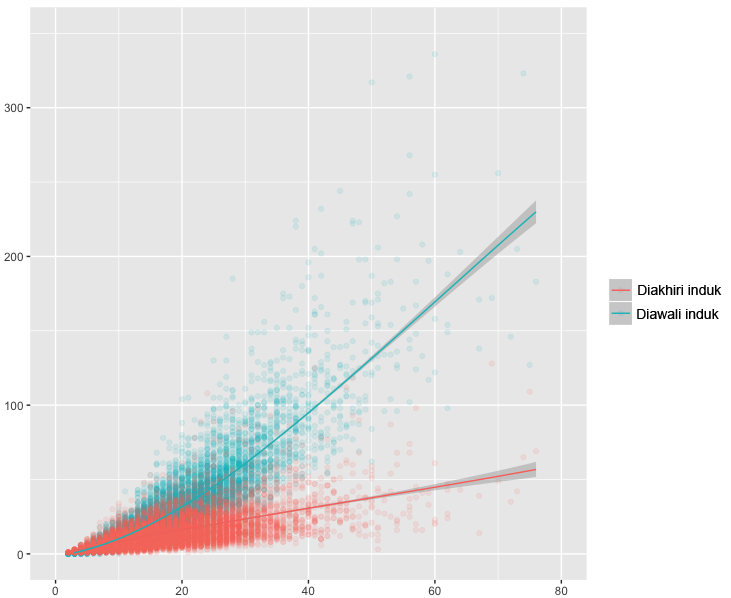
\includegraphics[width=1
	\textwidth] {pics/tulis_DLposneg.png} 
	\caption{Grafik nilai DL positif dan negatif data ragam tulis}
	\label{fig:tulis_DLposneg} 
\end{figure}

\begin{figure}
	\centering 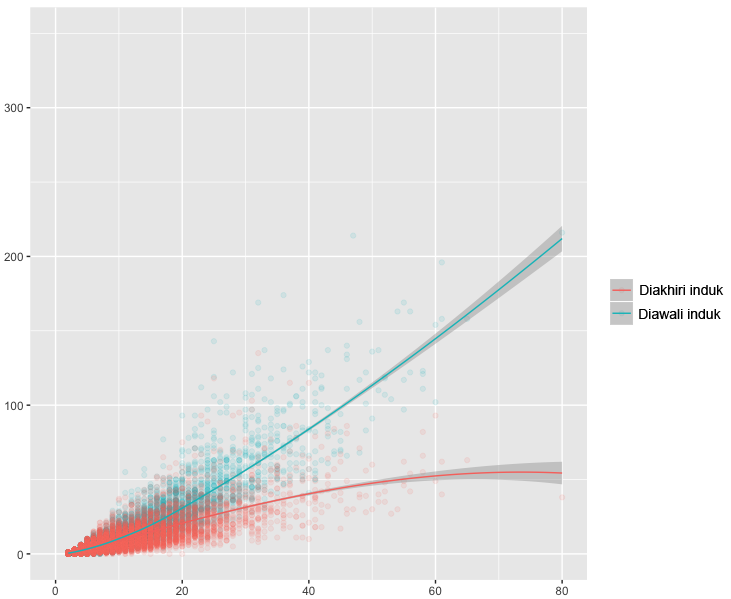
\includegraphics[width=1
	\textwidth] {pics/lisan_DLposneg.png} 
	\caption{Grafik nilai DL positif dan negatif data ragam tulis}
	\label{fig:lisan_DLposneg} 
\end{figure}

Pada bagian pertama analisis nilai DL positif dan negatif (\pic~\ref{fig:tulis_DLposneg}) dan \pic~\ref{fig:lisan_DLposneg}), kedua jenis nilai didapatkan dengan memisahkan total nilai dependensi positif dan negatif pada setiap kalimat. Nilai DL positif dan negatif ini memberikan gambaran kasus tautan root atau head dengan dependant secara general dan berkontribusi untuk membentuk asumsi kecenderungan karakteristik bahasa dilihat dari posisi head-nya (Wang & Liu, 2017). Berdasarkan \pic~\ref{fig:tulis_DLposneg} dan \pic~\ref{fig:lisan_DLposneg}, kedua korpus data menunjukkan garis regresi tautan dependensi positif yang jauh berada di atas garis regresi tautan dependensi negatif. Hal ini berarti ada pola kecenderungan preferensi terhadap hubungan root atau head sebelum dependant (head-initial). Seperti yang dijelaskan sebelumnya, nilai DL cukup sensitif terhadap panjang kalimat. Namun, terutama pada grafik nilai DL ragam lisan (\pic~\ref{fig:lisan_DLposneg}), garis regresi tautan dependensi negatif menunjukkan adanya kurva parabola terbalik sehingga muncul dugaan awal adanya ambang batas (threshold) terhadap nilai DL pada korpus data ragam lisan. Berdasarkan korpus data yang terkumpul, dugaan ambang batas tautan dependensi negatif ini menandakan bahwa mulai panjang kalimat tertentu, total tautan dependensi negatif dalam sebuah kalimat mungkin tidak akan melebihi nilai tertentu. 

\begin{figure}
	\centering 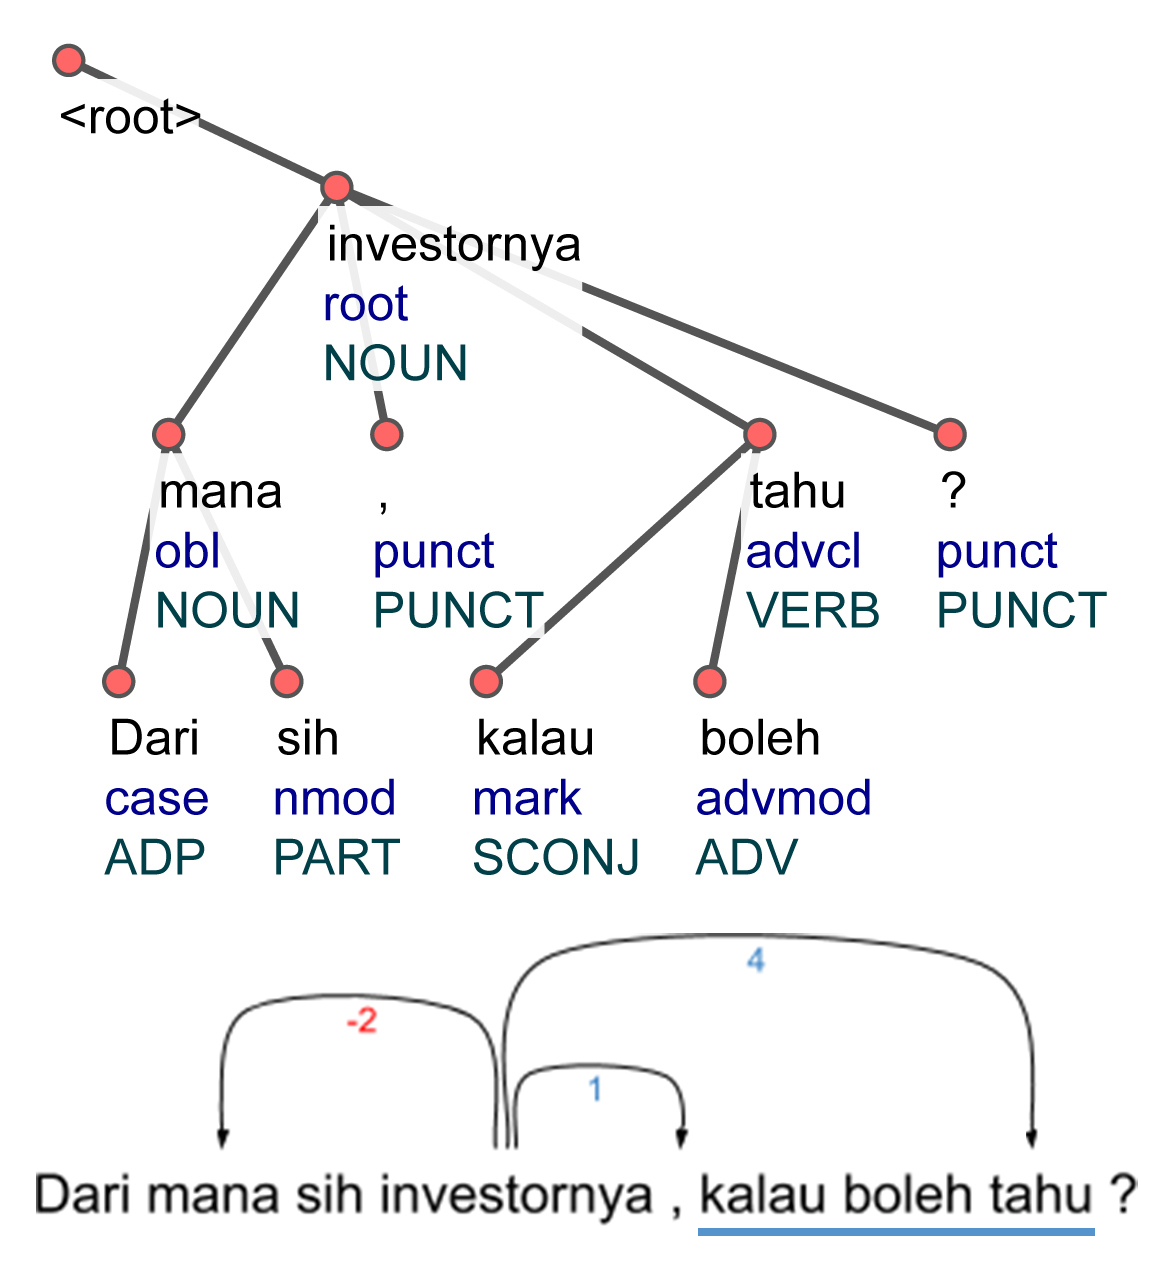
\includegraphics[width=1
	\textwidth] {pics/ls1436.jpg} 
	\caption{Kalimat L\textit{root}a pada data ragam lisan}
	\label{fig:ls1436} 
\end{figure}

\begin{figure}
	\centering 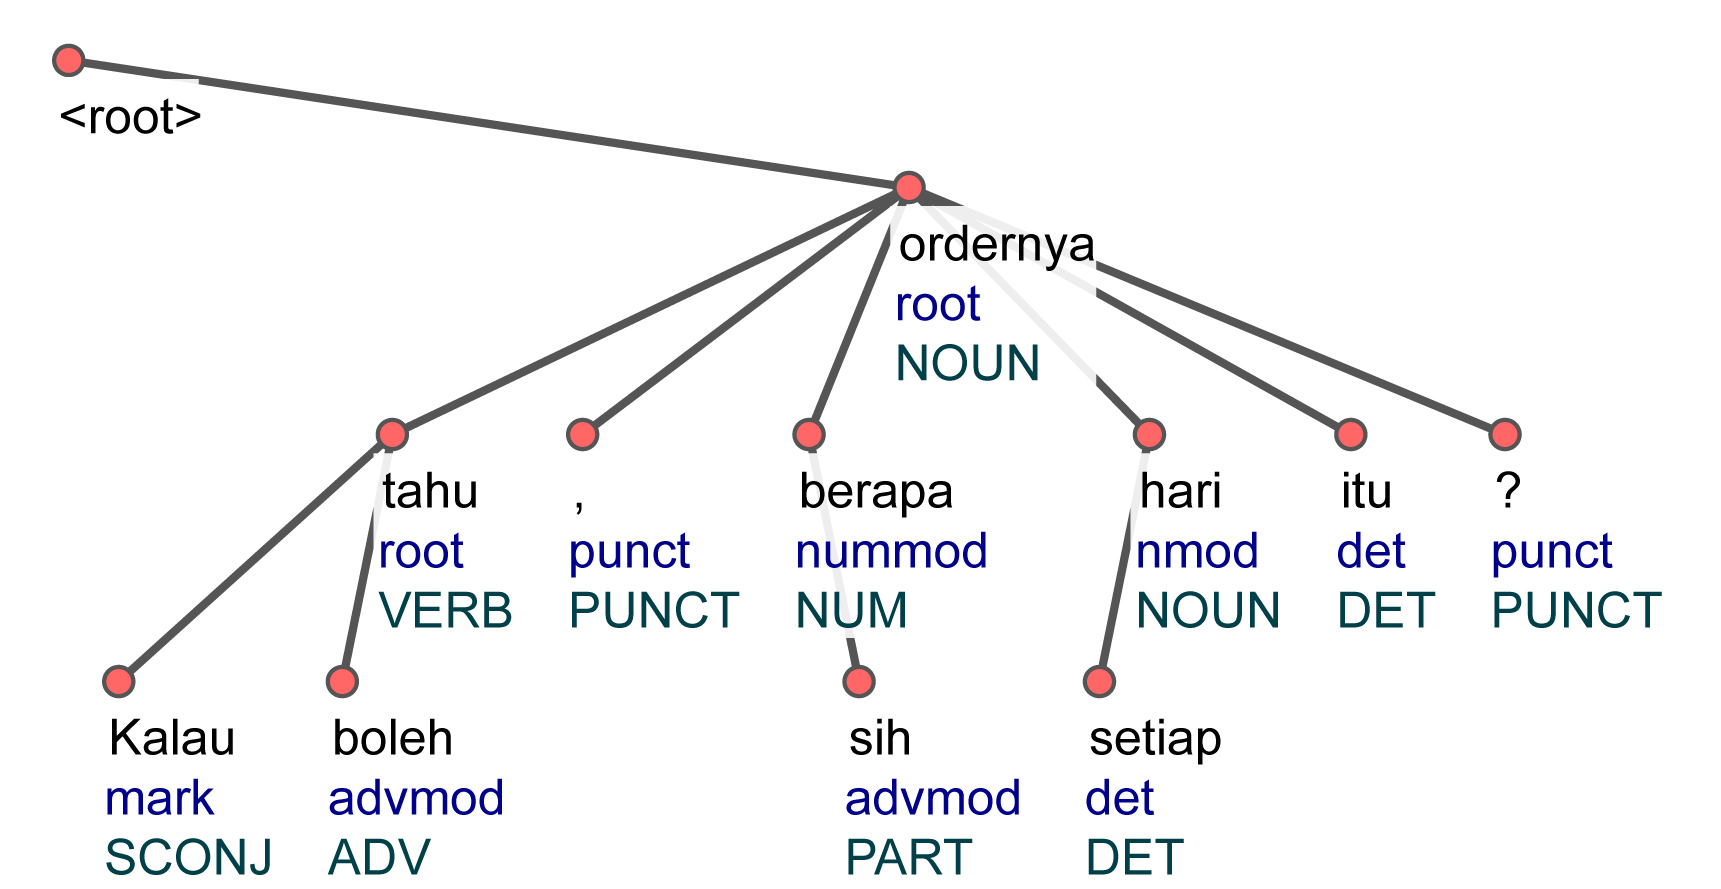
\includegraphics[width=1
	\textwidth] {pics/ls1460.jpg} 
	\caption{Kalimat L\textit{root}b pada data ragam lisan}
	\label{fig:ls1460} 
\end{figure}

\pic~\ref{fig:ls1436} dan \pic~\ref{fig:ls1460} merupakan perbandingan kedua kalimat yang ditemukan pada korpus data ragam lisan. Gambar ini memberikan ilustrasi perbedaan letak root dan dampaknya terhadap nilai dependensi. Klausa terikat "kalau boleh tahu" pada kalimat L\textit{root}a dan L\textit{root}b berada pada posisi yang berbeda. Pada kalimat L\textit{root}b, kata-kata yang membentuk "kalau boleh tahu" secara kolektif memiliki hubungan dependensi utama negatif terhadap root "ordernya". Berdasarkan teori dependensi yang dijabarkan oleh Tesniere (1959), klausa terikat pada posisi awal ujaran ini harus disimpan dalam memori kerja terlebih dahulu hingga root direalisasikan. Hal in berkebalikan dengan L\textit{root}a yang dapat diproses langsung karena root sudah direalisasikan terlebih dahulu.

\begin{figure}
	\centering 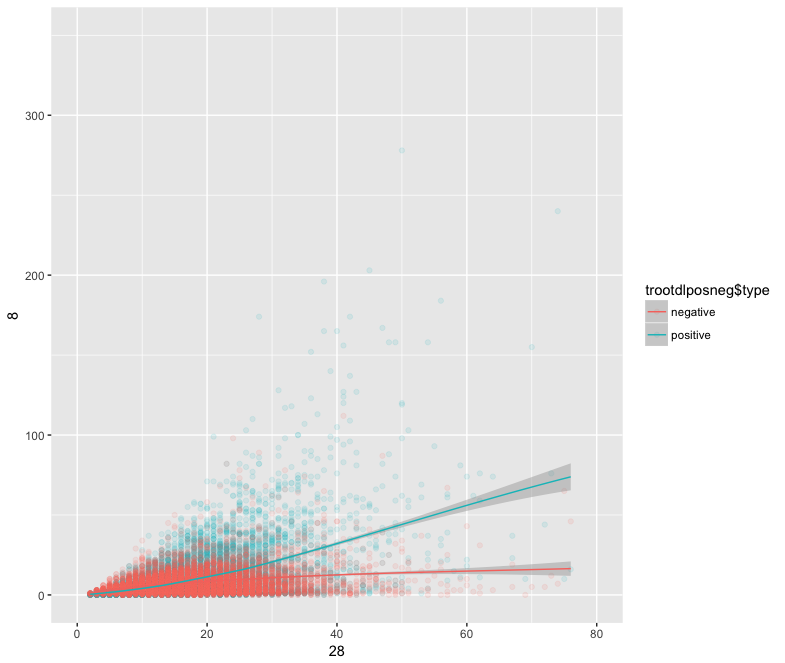
\includegraphics[width=1
	\textwidth] {pics/tulisroot_DLposneg.png} 
	\caption{Grafik nilai DL positif dan negatif pada simpai sentral dengan root berupa verba data ragam tulis}
	\label{fig:tulisroot_DLposneg} 
\end{figure}

\begin{figure}
	\centering 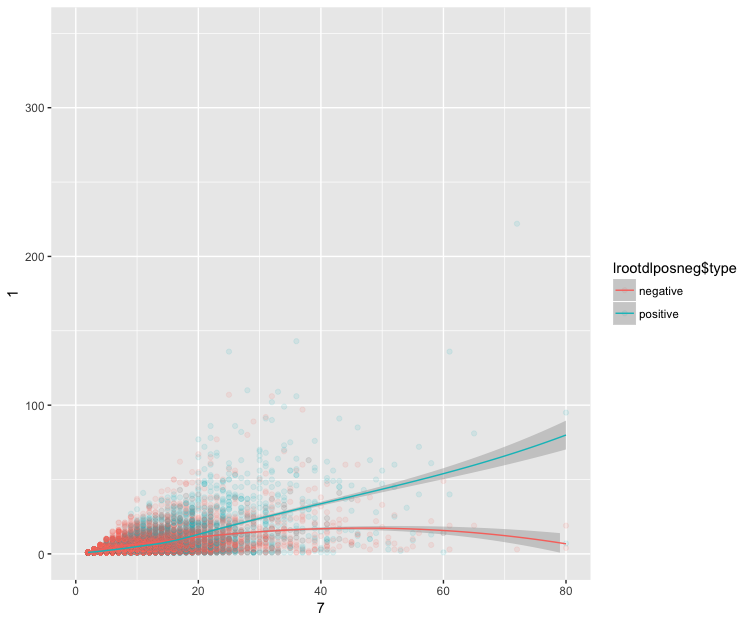
\includegraphics[width=1
	\textwidth] {pics/lisanroot_DLposneg.png} 
	\caption{Grafik nilai DL positif dan negatif pada simpai sentral dengan root berupa verba data ragam lisan}
	\label{fig:lisanroot_DLposneg} 
\end{figure}

Bagian kedua analisis nilai DL positif dan negatif berkaitan dengan valensi sebuah kata. Sesuai dengan batasan penelitian ini, bagian analisis ini difokuskan hanya pada simpai sentral dengan kelas kata root berupa verba. \pic~\ref{fig:tulisroot_DLposneg} dan \pic~\ref{fig:lisanroot_DLposneg} merupakan grafik nilai DL positif dan negatif  yang didapat hanya pada simpai sentral ujara dengan root berupa verba. Ujaran dengan root verbal ditemukan sebanyak 84,67\% atau sebanyak 7884 ujaran pada data ragam tulis dan 69,26\% atau sebanyak 7078 ujaran pada data ragam lisan. Mayoritas root verbal ini dapat dianalisis untuk melihat bagaimana penutur menyusun informasi utama dengan melihat tautan-tautan dependensi utama (simpai sentral). Sehingga, semua klausa yang mungkin terikat pada simpai cabang dianggap mengikuti head-nya. Gambar 12 menunjukkan bahwa pada level tautan dependensi utama, penutur juga cenderung memilih untuk menekan nilai dependensi negatif. Serupa dengan Gambar 0, terutama pada data ragam lisan, garis regresi nilai DL negatif mengindikasikan adanya threshold pada nilai tertentu. 	

%%-----------------------------------------------------------------------------%
\subsection{Temuan 6: Penempatan root verbal dan/atau klausa bebas utama di awal ujaran tanpa pengurangan valensi verbal}
%%-----------------------------------------------------------------------------%
Penempatan root dan/atau klausa bebas utama di awal ujaran tanpa mengurangi valensi verbal sangat banyak ditemukan pada kedua korpus data. Penempatan root verbal pada posisi pertama seperti kalimat Troota dan Trootb (Gambar 13) cukup banyak ditemukan pada semua klasifikasi dalam korpus data ragam tulis klasifikasi kalimat pendek dan menengah. Sebaliknya, penempatan root di posisi pertama tanpa mengurangi valensi verbal tersebut sangat jarang ditemukan pada data ragam lisan.

\begin{figure}
	\centering 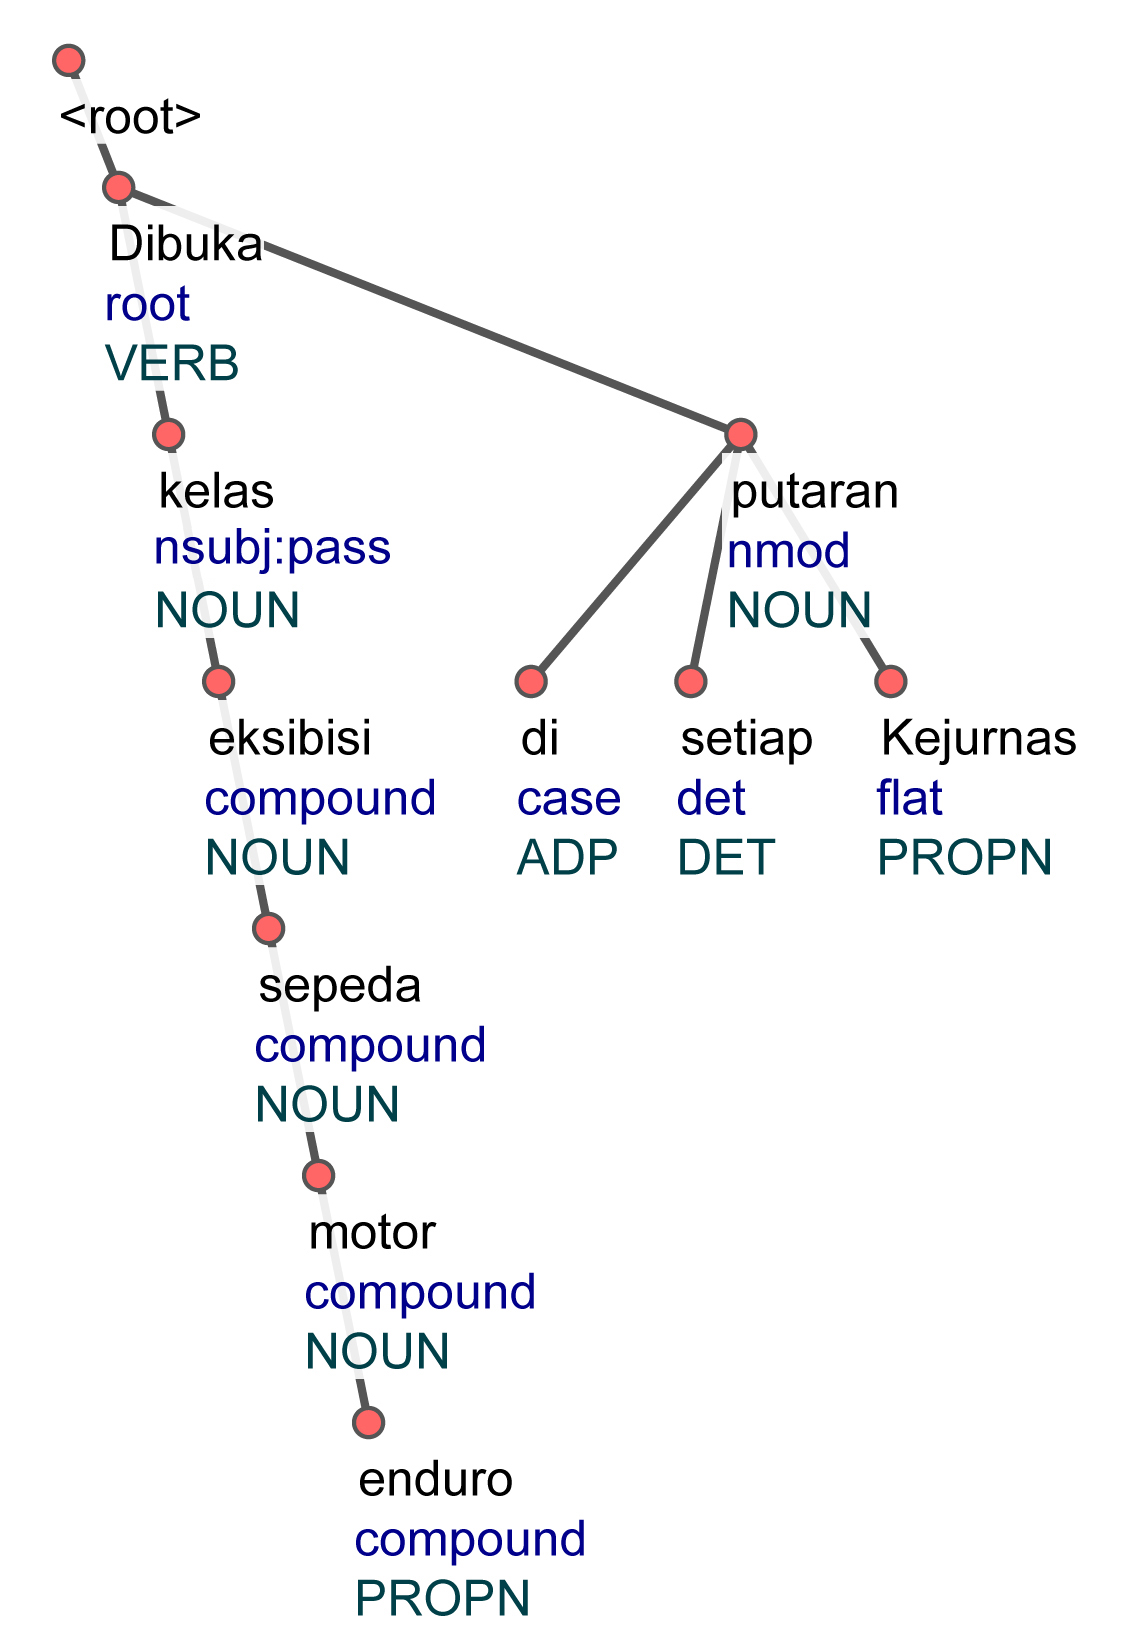
\includegraphics[width=1
	\textwidth] {pics/ts770.jpg} 
	\caption{Kalimat Troota pada data ragam tulis}
	\label{fig:ts770} 
\end{figure}

\begin{figure}
	\centering 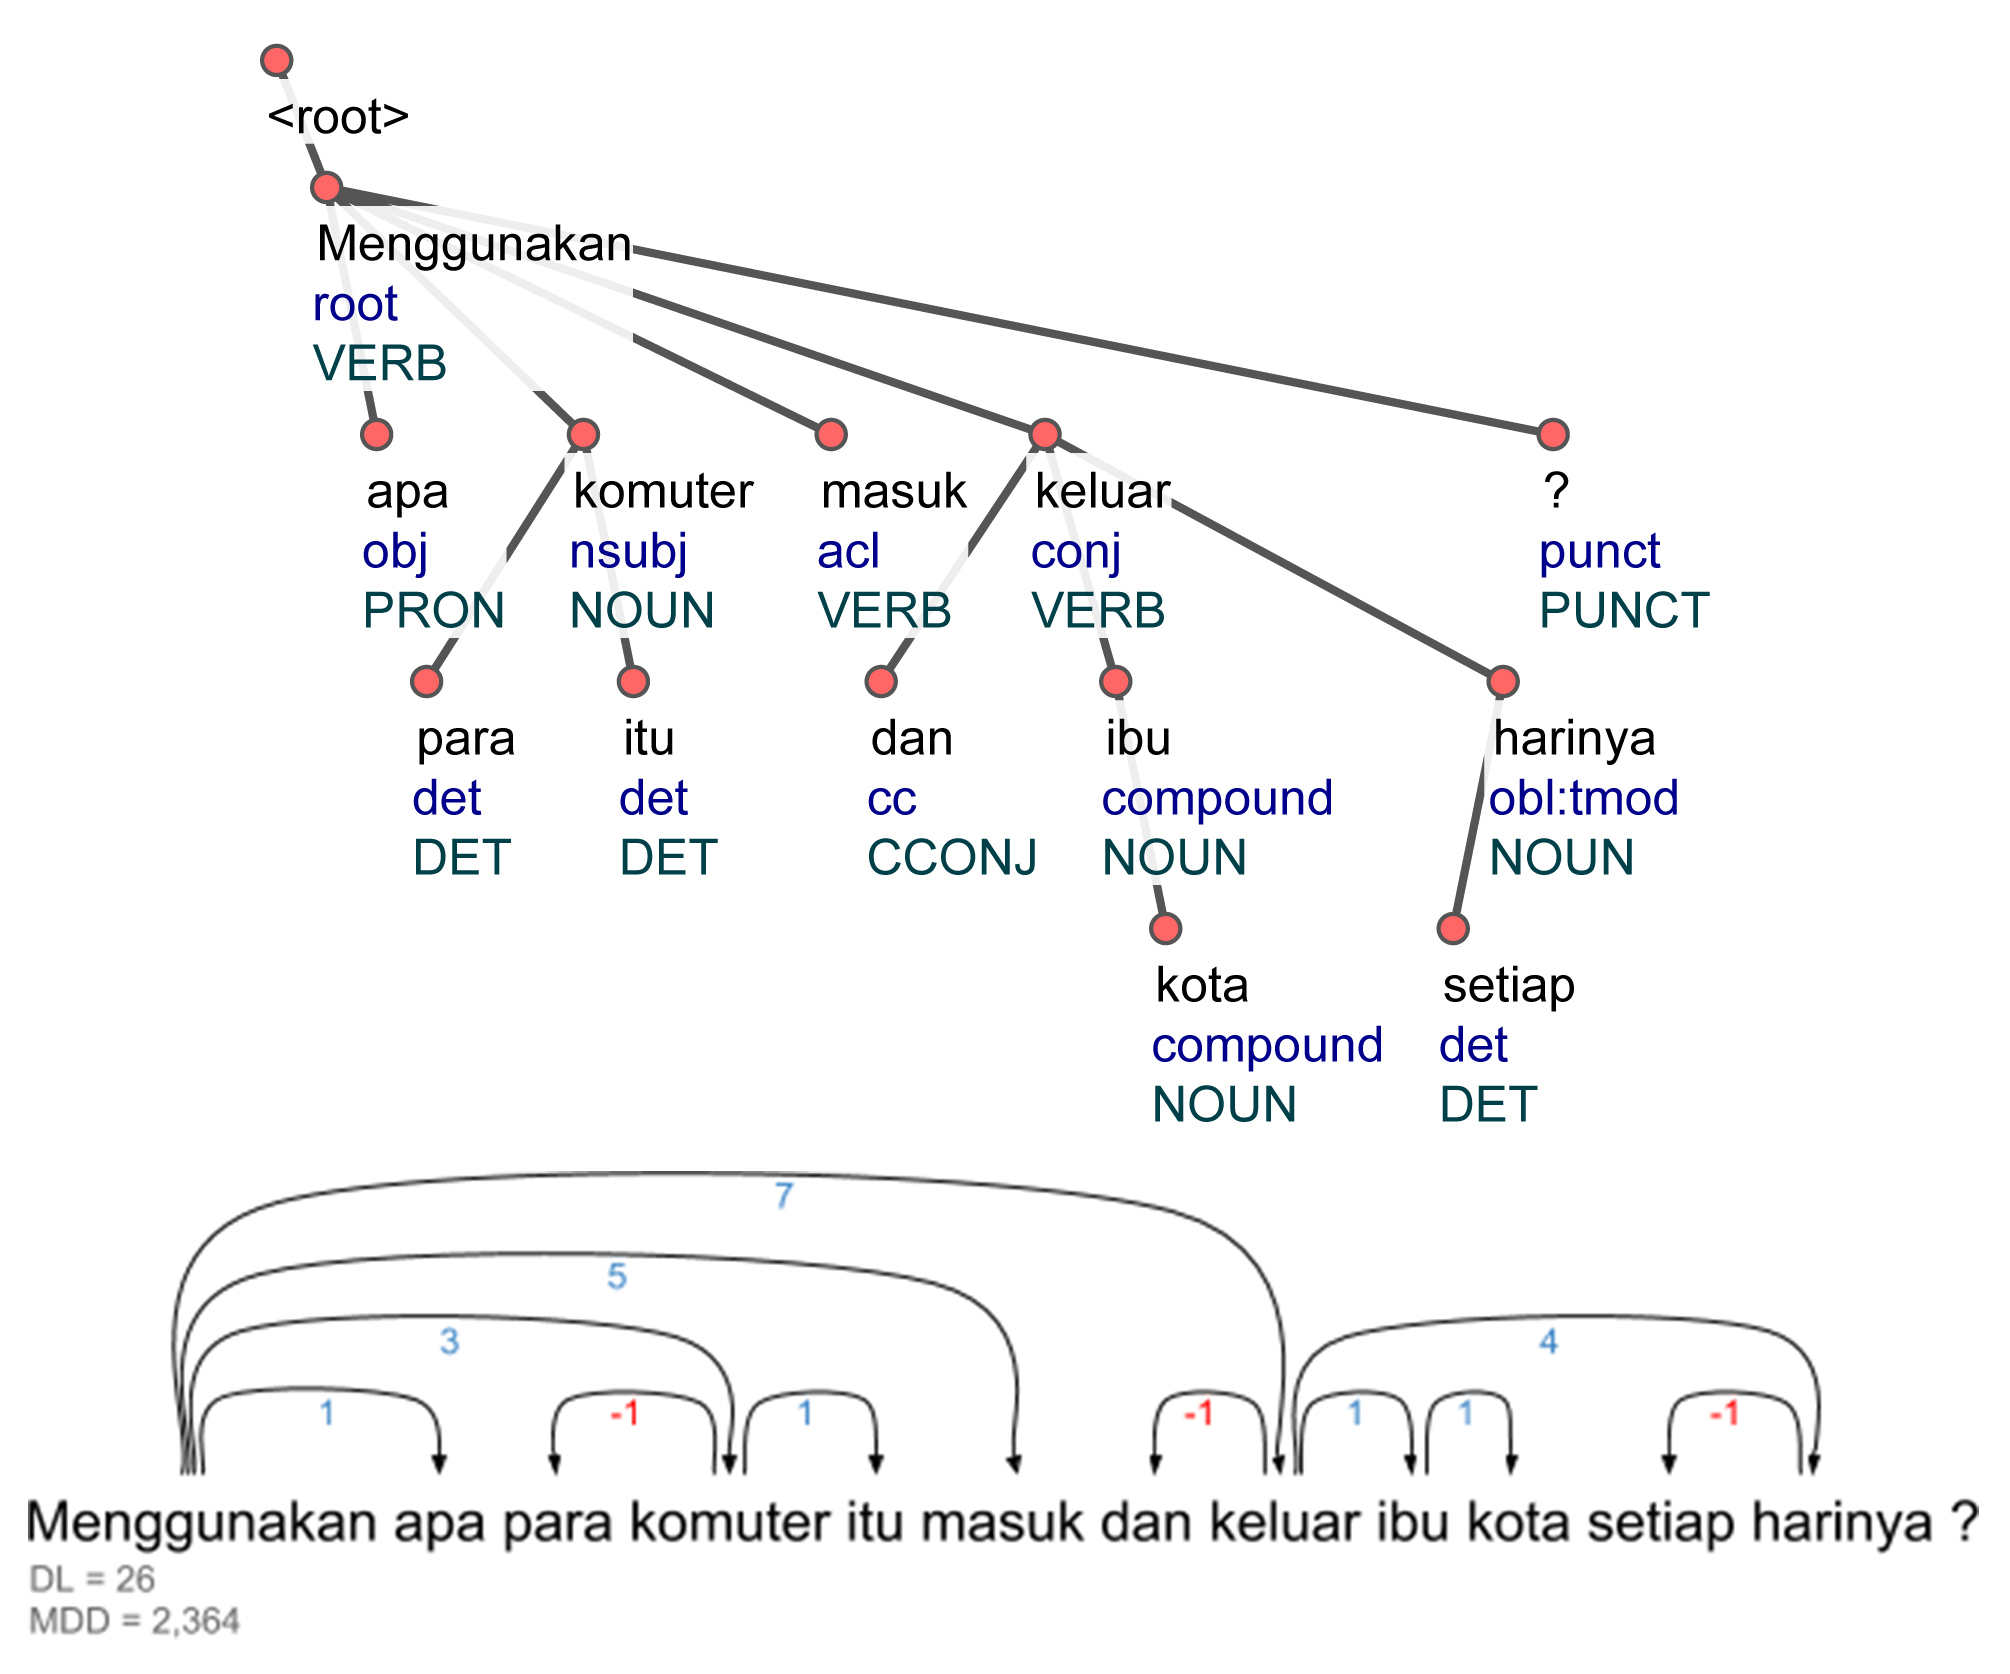
\includegraphics[width=1
	\textwidth] {pics/ts7458.jpg} 
	\caption{Kalimat Trootb pada data ragam tulis}
	\label{fig:ts7458} 
\end{figure}

Pada kalimat Troota, root verbal "dibuka" tetap mengikat dependant "kelas". Kata "dibuka" pada kalimat Troota tergolong verba statif (keadaan) sehingga tidak diperlukan kemunculan aktor pelaku dalam kalimat terebut (Sneddon, 2010). Serupa dengan kalimat Troota, root verbal "menggunakan" pada kalimat Trootb tetap mempertahankan valensi terhadap "komuter" (aktor pelaku) dan "apa" (pengganti obyek). Contoh ini memberikan indikasi pemanfaatan kebebasan urutan kata dalam Bahasa Indonesia untuk menghindari tautan dependensi negatif dengan merealisasikan root seawal mungkin. Pada data ragam tulis dan lisan klasifikasi kalimat panjang, penempatan klausa bebas utama di awal ujaran menyebabkan secara otomatis root verbal tetap cenderung berada di awal ujaran, tanpa mengurangi valensi verbal root tersebut. Namun, karena jumlah konstituen yang panjang dan struktur kalimat dengan klausa-klausa yang lebih kompleks, posisi root verbal umumnya tidak pada tiga posisi pertama. Contoh strategi ini dapat dilihat pada kalimat T31b (\pic~\ref{fig:}, dan \pic~\ref{fig:}) untuk data ragam tulis dan L31a (\pic~\ref{fig:},\pic~\ref{fig:}, dan \pic~\ref{fig:}) untuk data ragam lisan.

%%-----------------------------------------------------------------------------%
\subsection{Temuan 7: Penempatan root verbal dan klausa bebas di awal ujaran disertai pengurangan valensi verbal}
%%-----------------------------------------------------------------------------%
Sejumlah simpai sentral dalam kedua korpus data mengalami pengurangan valensi verbal yang mengakibatkan pengurangan panjang serta jarak dependensi. Ujaran seperti ini sangat jarang ditemui pada data ragam tulis, cukup banyak ditemukan pada data ragam lisan, terutama pada klasifikasi kalimat pendek dan menengah. Strategi pengurangan valensi verbal ini banyak ditemukan disertai dengan penempatan root di awal ujaran seperti pada temuan sebelumnya. 

\begin{figure}
	\centering 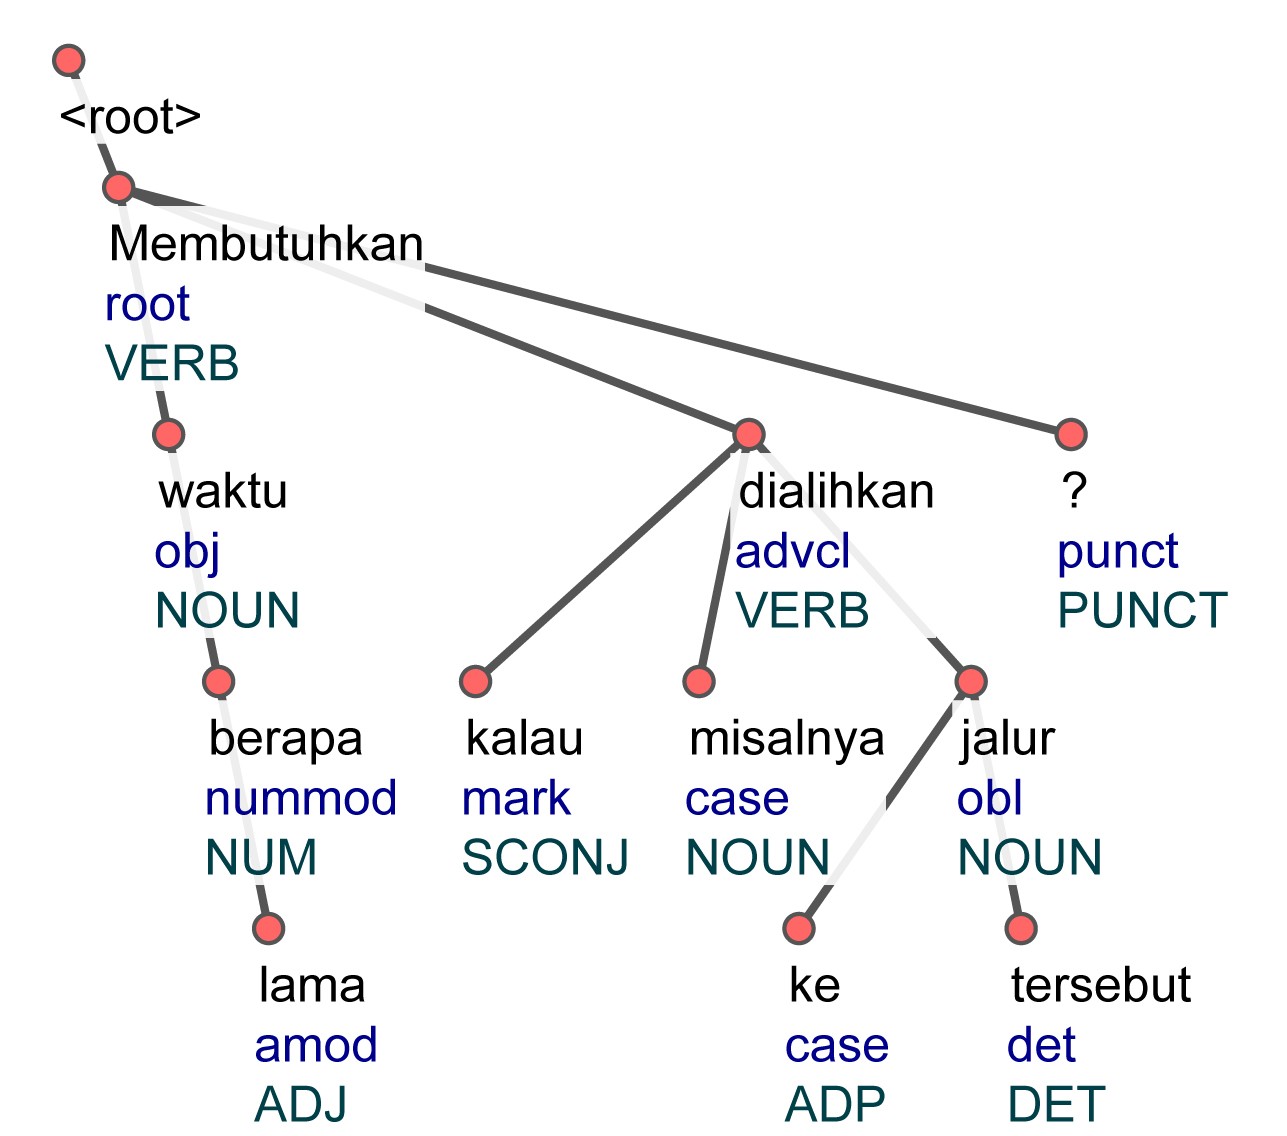
\includegraphics[width=1
	\textwidth] {pics/ls4820.jpg} 
	\caption{Kalimat Trootc pada data ragam tulis}
	\label{fig:ls4820} 
\end{figure}

\begin{figure}
	\centering 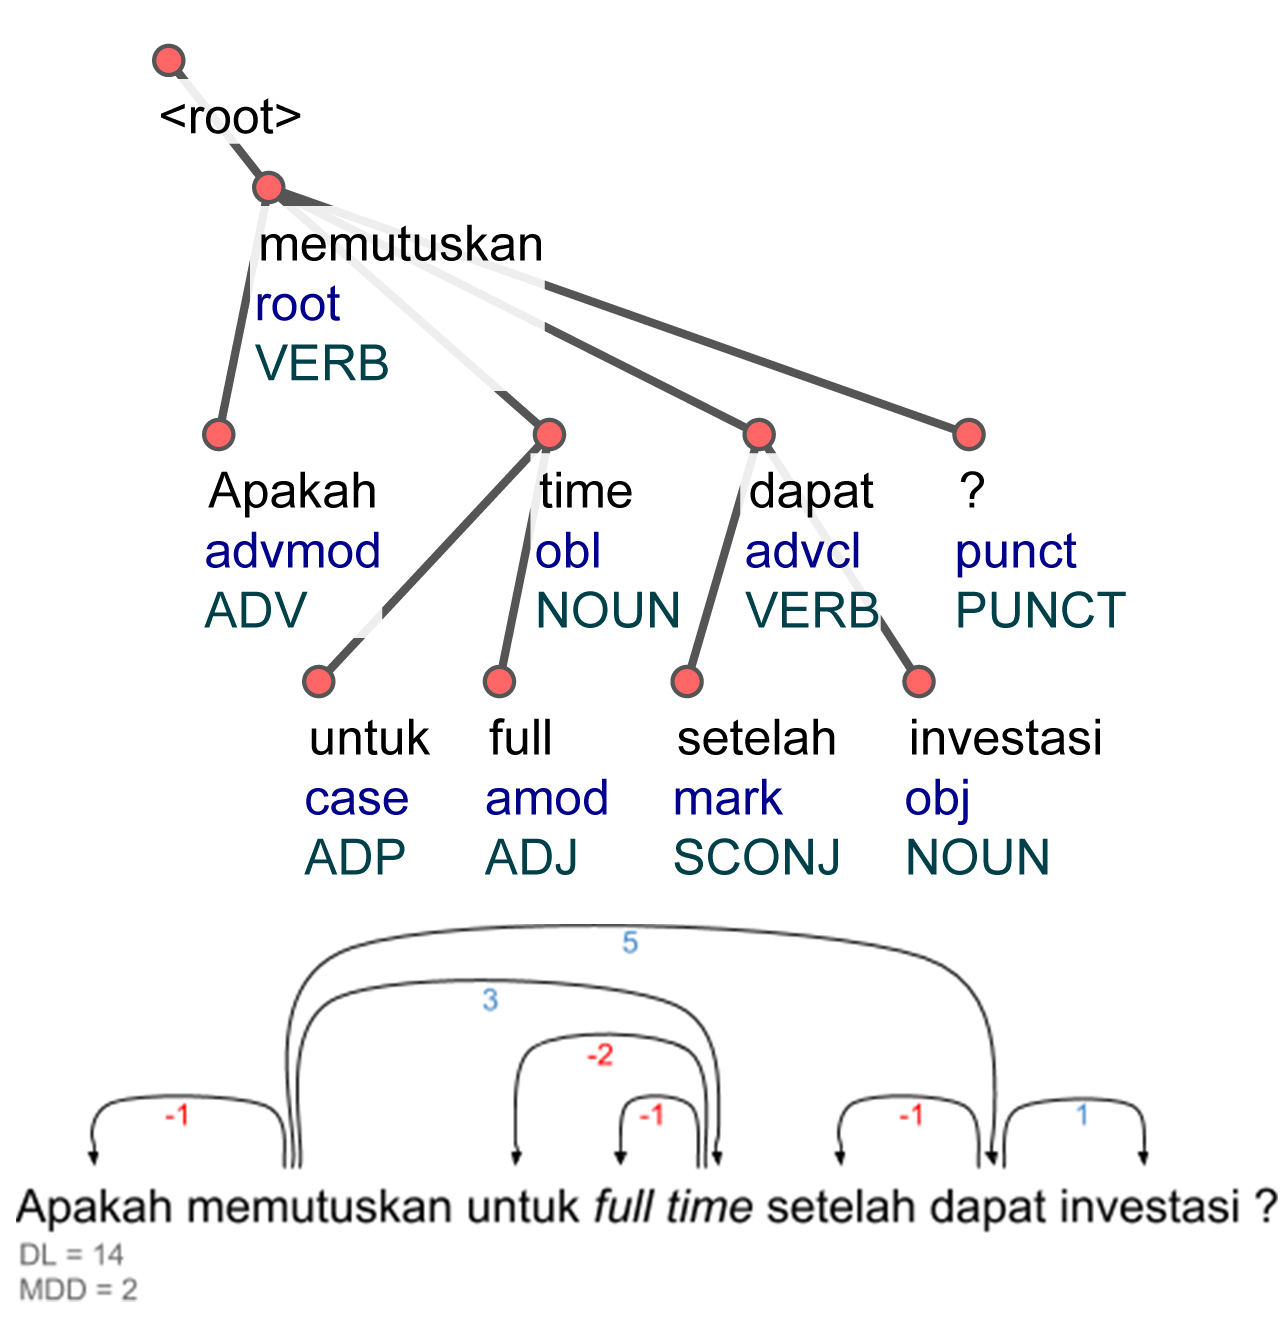
\includegraphics[width=1
	\textwidth] {pics/ls1435.jpg} 
	\caption{Kalimat Trootc pada data ragam tulis}
	\label{fig:ls1435} 
\end{figure}

Pada kalimat Lrootc (\pic~\ref{fig:ls4820}, dan \pic~\ref{fig:ls1435}), root verbal "membutuhkan" umumnya memiliki valensi sebanyak dua kata, yaitu aktor pelaku dan obyek  atau "(X) membutuhkan (Y)". Kata ini mengalami pengurangan valensi verbal sehingga yang muncul hanya obyek. Begitu pula dengan kalimat Lrootd yang sama-sama mengalami pengurangan valensi verbal berupa aktor pelaku. Kalimat Lroote (\pic~\ref{fig:}) juga tidak memunculkan aktor pelaku yang dapat melengkapi salah satu valensi root verbal pada klausa bebas "(X) mengganti alat" ataupun valensi head verbal pada klausa terikat "supaya (X) tidak berebut ikan".

\begin{figure}
	\centering 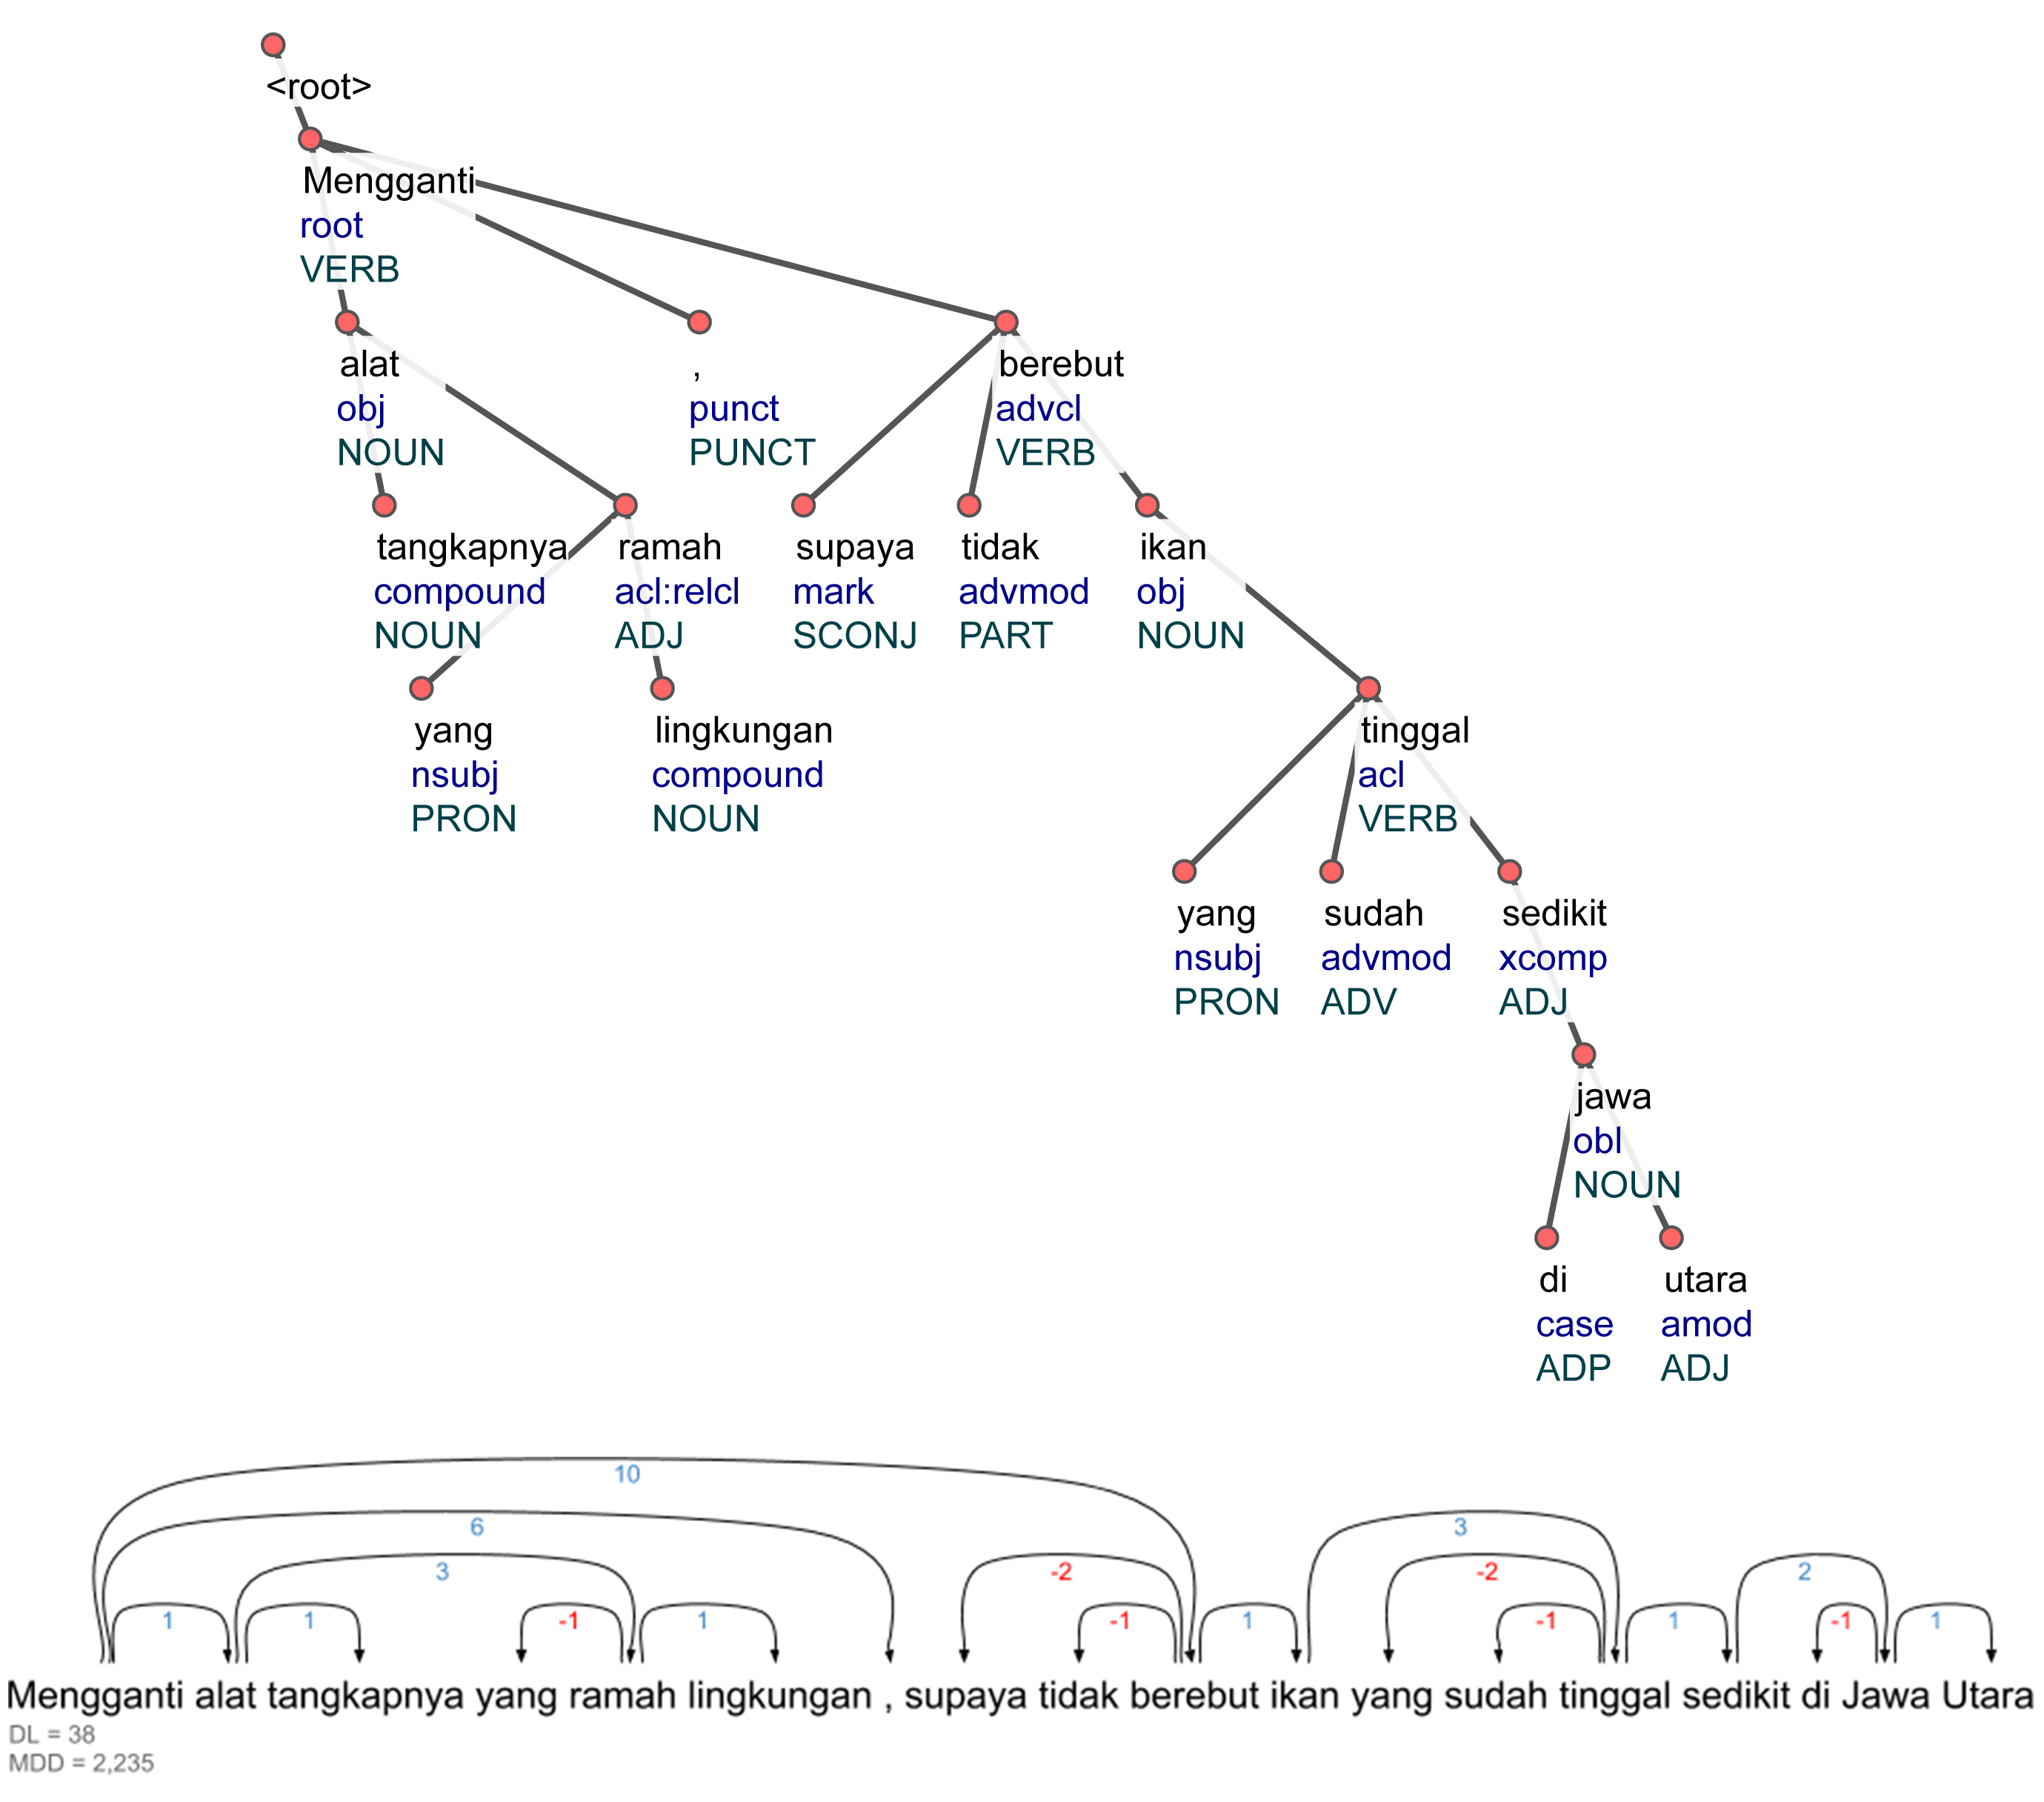
\includegraphics[width=1
	\textwidth] {pics/ls1265.jpg} 
	\caption{Kalimat Lroote pada data ragam lisan}
	\label{fig:ls1265} 
\end{figure}

Strategi ujaran seperti ini muncul dalam wacana-wacana di mana konstituen yang direduksi dari valensi verbal sudah terlebih dahulu direalisasikan di ujaran-ujaran sebelumnya atau sudah dimengerti bersama tanpa harus direalisasikan dalam kalimat tertentu. Cakupan penelitian ini hanya pada tataran kalimat sehingga tidak menganalisis hubungan dependensi yang terbentuk antarkalimat. Namun, asumsi ini menimbulkan pertanyaan analisis dependensi lanjutan pada tataran wacana yaitu bagaimana dan sejauh mana tautan dependensi yang terbentuk antarkalimat sehingga memungkinkan adanya pengurangan valensi verbal pada kalimat tertentu?

%%-----------------------------------------------------------------------------%
\subsection{Diskusi temuan 6 dan 7}
%%-----------------------------------------------------------------------------%
Bagian analisis ini mencoba menjawab pertanyaan terkait arah tautan dependensi dan peengurangan valensi verbal pada simpai sentral. Pengurangan kata dalam kalimat atau preferensi terhadap kalimat pendek terutama pada ragam lisan tidak selalu berarti menandakan adanya pengurangan valensi. Pada penelitian-penelitian terdahulu banyak dilakukan eksplorasi terhadap reduksi leksikal lain seperti konjungsi, partikel, ataupun kata-kata lain yang berulang (Jaeger, 2006; Gildea & Temperley, 2015). Penelitian ini memfokuskan pada simpai sentral dengan root verbal yang merupakan jenis root yang paling banyak ditemukan pada kedua korpus data. 

Seperti yang dibahas pada bab sebelumnya, arah tautan dependensi dapat menyebabkan nilai dependensi tersebut menjadi positif atau negatif. Nilai positif yang menandakan bentuk head-initial dianggap lebih memudahkan proses memori kerja karena konstituen induk (head) yang mengandung informasi utama sudah direalisasikan terlebih dahulu. Meskipun begitu, bentuk head-intial tidak selalu menjadi preferensi pada semua bahasa karena beberapa bahasa memiliki aturan tata bahasa yang menuntut head muncul setelah konstituen terikat (dependant) atau head-final. Berdasarkan aturan struktur frasa dalam tata bahasa yang ada (Kridalaksana, 2002; Sneddon, 2010), terdapat indikasi bahwa Bahasa Indonesia tergolong bahasa yang memilih bentuk head-initial dibandingkan head-final. Namun, belum ada penelitian dengan skala cukup besar yang dapat memberikat informasi ini dengan memanfaatkan data ujaran nyata (real utterance) karena penerapannya dalam ujaran nyata dapat bersifat tidak gramatikal.  Berdasarkan data hasil observasi penelitian ini, temuan yang didapat mendukung asumsi bahwa ada preferensi terhadap bentuk head-initial yang ditandai oleh konsistensi nilai DL positif yang semakin tinggi seiring jumlah konstituen yang semakin banyak. Secara otomatis pergerakan nilai DL positif yang semakin tinggi mengakibatkan penekanan nilai DL negatif. Kedua korpus data menunjukkan bahwa dalam 1 ujaran, ada kecenderungan untuk mengurangi tautan dependensi negatif dan temuan ini ditemukan pada kedua bagian analisis (antarkonstituen yang memiliki tautan langsung maupun antarkonstituen pada simpai sentral). Temuan ini menandakan konsistensi untuk menekan nilai DL negatif pada level struktur yang berbeda dan mengindikasikan preferensi head-initial di segala kondisi. 

Analisis kualitatif untuk melihat lebih dalam bagaimana strategi yang mendukung preferensi head-initial ini dilakukan dengan mencermati simpai-simpai sentral ujaran yang memiliki root verbal pada kedua korpus. Secara umum, ditemukan dua strategi terkait arah dan valensi kata yaitu, penempatan root dan/atau klausa bebas utama di awal ujaran dengan atau tanpa mengurangi valensi konstituen induk. Penempatan root dan/atau klausa bebas utama di awal ujaran sangat umum ditemukan pada semua klasifikasi dalam korpus data ragam tulis. Namun, posisinya sedikit bergeser seiring dengan semakin banyaknya jumlah konstituen. Hal ini dikarenakan penempatan klausa bebas utama yang hampir selalu di posisi awal pada data ragam tulis. Sementara, pengurangan valensi root verbal hampir tidak ditemukan pada data ragam tulis yang mungkin disebabkan karena karakter wacananya lebih formal dibandingkan dengan ragam lisan. Pengurangan valensi ini secara langsung berakibat pada pengurangan konstituen secara keseluruhan, sehingga dapat dikaitkan dengan temuan adanya preferensi untuk kalimat dengan jumlah konstituen yang lebih sedikit pada ragam lisan. Pengurangan valensi root verbal ini sering disertai dengan penempatan posisi root di awal ujaran ragam lisan namun hampir tidak ditemukan pada klasifikasi kalimat panjang. 

Pada klasifikasi kalimat pendek dan menengah data ragam tulis, penempatan root verbal sering berada pada posisi pertama hingga ketiga dan disertai pengurangan aktor pelaku atau subyek yang (secara tata bahasa) umumnya mendahului verba tersebut. Pengurangan valensi berupa aktor pelaku atau subyek pada simpai dengan induk berupa verba tidak ditemukan apabila klausa tersebut didahului klausa lain. Temuan pengurangan aktor pelaku atau subyek hanya pada awal ujaran ini mungkin diakibatkan oleh hubungan antarkalimat yang menuntut penelitian di luar batasan penelitian ini. 

%%-----------------------------------------------------------------------------%
%\section{thesis.tex}
%%-----------------------------------------------------------------------------%
%Berkas ini berisi seluruh berkas Latex yang dibaca, jadi bisa dikatakan sebagai 
%berkas utama. Dari berkas ini kita dapat mengatur bab apa saja yang ingin 
%kita tampilkan dalam dokumen.
%
%
%%-----------------------------------------------------------------------------%
%\section{laporan\_setting.tex}
%%-----------------------------------------------------------------------------%
%Berkas ini berguna untuk mempermudah pembuatan beberapa template standar. 
%Anda diminta untuk menuliskan judul laporan, nama, npm, dan hal-hal lain yang 
%dibutuhkan untuk pembuatan template. 
%
%
%%-----------------------------------------------------------------------------%
%\section{istilah.tex}
%%-----------------------------------------------------------------------------%
%Berkas istilah digunakan untuk mencatat istilah-istilah yang digunakan. 
%Fungsinya hanya untuk memudahkan penulisan.
%Pada beberapa kasus, ada kata-kata yang harus selalu muncul dengan tercetak 
%miring atau tercetak tebal. 
%Dengan menjadikan kata-kata tersebut sebagai sebuah perintah \latex~tentu akan 
%mempercepat dan mempermudah pengerjaan laporan. 
%
%
%%-----------------------------------------------------------------------------%
%\section{hype.indonesia.tex}
%%-----------------------------------------------------------------------------%
%Berkas ini berisi cara pemenggalan beberapa kata dalam bahasa Indonesia. 
%\latex~memiliki algoritma untuk memenggal kata-kata sendiri, namun untuk 
%beberapa kasus algoritma ini memenggal dengan cara yang salah. 
%Untuk memperbaiki pemenggalan yang salah inilah cara pemenggalan yang benar 
%ditulis dalam berkas hype.indonesia.tex.
%
%
%%-----------------------------------------------------------------------------%
%\section{pustaka.tex}
%%-----------------------------------------------------------------------------%
%Berkas pustaka.tex berisi seluruh daftar referensi yang digunakan dalam 
%laporan. 
%Anda bisa membuat model daftar referensi lain dengan menggunakan bibtex.
%Untuk mempelajari bibtex lebih lanjut, silahkan buka 
%\url{http://www.bibtex.org/Format}. 
%Untuk merujuk pada salah satu referensi yang ada, gunakan perintah \bslash 
%cite, e.g. \bslash cite\{latex.intro\} yang akan akan memunculkan 
%\cite{latex.intro}
%
%
%%-----------------------------------------------------------------------------%
%\section{bab[1 - 6].tex}
%%-----------------------------------------------------------------------------%
%Berkas ini berisi isi laporan yang Anda tulis. 
%Setiap nama berkas e.g. bab1.tex merepresentasikan bab dimana tulisan tersebut 
%akan muncul. 
%Sebagai contoh, kode dimana tulisan ini dibaut berada dalam berkas dengan nama 
%bab4.tex. 
%Ada enam buah berkas yang telah disiapkan untuk mengakomodir enam bab dari 
%laporan Anda, diluar bab kesimpulan dan saran. 
%Jika Anda tidak membutuhkan sebanyak itu, silahkan hapus kode dalam berkas 
%thesis.tex yang memasukan berkas \latex~yang tidak dibutuhkan;  contohnya 
%perintah \bslash include\{bab6.tex\} merupakan kode untuk memasukan berkas 
%bab6.tex kedalam laporan.
%
